\documentclass[12 pt, a4paper]{article}
\usepackage[english]{babel}  								% For norsk oppsett
\usepackage[utf8]{inputenc}
\usepackage{amsmath}
\usepackage{amssymb}
\usepackage{graphicx}
\usepackage{tabularx}
\usepackage{subcaption}
\usepackage{hyperref}
\usepackage{fancyhdr}
\usepackage{enumerate}
\usepackage{float}
\usepackage{tikz}
\usepackage{fancyhdr}
\usepackage{lastpage}
\usepackage{circuitikz}
\usepackage{physics}
\usepackage[includeheadfoot, margin =0.5 in]{geometry}
\usepackage[FYS, OnlyFrontpage]{mnfrontpage} 			%SKIFT HER!!!
\usepackage[version=3]{mhchem}
\usepackage{biblatex}%,style=numeric-comp
%\usepackage{cite}
\usepackage{siunitx}
\usepackage{todonotes}
\usepackage{xcolor}
\usepackage{listings}
%%%%
\usepackage[bottom]{footmisc}
\renewcommand\footnoterule{\rule{\linewidth}{0.5pt}}
%\renewcommand[\footnoterule]{%
%	\kern -3pt
%	\hrule width \textwidth height 1pt 
%	\kern 2pt
%}
%%%%
\lstset{basicstyle=\ttfamily,
  showstringspaces=false,
  commentstyle=\color{red},
  keywordstyle=\color{blue}
}
%\usepackage{showframe}  %Dette viser hvordan strukturen på sidene er

\setlength{\parindent}{0cm}

\author{
\href{https://scontent.fosl1-1.fna.fbcdn.net/v/t31.0-8/12671762_10153383742266712_8474119290530634136_o.jpg?oh=22ee31dac1e3bff8a581f96848315dbc&oe=5A7942F3}{Erik Skaar}
}



\bibliography{kilder.bib}






\font\myfont=cmr12 at 35pt
\title{\textbf{{\myfont Monte Carlo Modeling of Transactions}}}
\begin{document}
\mnfrontpage


\pagestyle{fancy}
\fancyhf{}
\rhead{FYS4150}
\lhead{\href{https://github.com/erikfsk/Project-3}{Erik Skaar}}
\fancyfoot[CE,LO]{\leftmark}
\fancyfoot[LE,RO]{Page \number\value{page} of \pageref{LastPage}}

\renewcommand{\headrulewidth}{2pt}
\renewcommand{\footrulewidth}{1pt}

\tableofcontents



\pagebreak
\section*{Abstract}%1

\abstract{I this project a model of a financial marked is build up from the basics, and follows two papers written on financial models. Three additional different levels of complexity is added to the system to expand the model. First the system only consists of agents that has to trade with each other. The resulting plots from this model is then compared to Pareto's law to verify the models basics. Then a savings term is introduced and several different savings factors are compared to make a comment on how saving influences the money distribution. Then a probability is added to the transaction stage. Here people with a similar amount of money are more willing to do a transaction. A scaling power factor is introduced and varied to influence to what extend the similarity in wealth influences the probability to trade. Here the results are commented and compared to Pareto's law. Finally a trust term is included in the probability term. This term increases the probability of making a transaction if the agents has previously done transactions. This term also has a scaling power factor which is varied to compare the influence of this term on the final wealth distribution. Lastly a modification is done to one of the scaling factors compared to the one in the papers followed in this project.}




\section{Introduction}
\section{Introduction}

Predictions of how the financial marked works has, in the modern age, become a large field of study\cite{publisher}. With the knowledge of how stock exchanges work can a mathematical model be build up to simulate these exchanges in the hope that one can predict prices and trends in the future. These predictions are in turn used as a basis for investments and such. The accuracy and speed of these models are therefore of the utmost importance. When these models predicts the wrong outcome things can go very wrong as it did in 2009\cite{marketcrash}.\\

In this project a simulation is done on a simple closed economy model. The economy model consists of a group of financial agents with the ability to transfer money between themselves, using the Monte Carlo method. The simulation will be compared to the well established Pareto's law \cite{paretoslaw}, and the analysis follows two papers. Patriarca with collaborates made one of the articles.\cite{patriarca} The second one was written by Goswami and Sen. \cite{goswami}

In the first simulation all financial agents are made equal and there is a $100\%$ probability of a transaction taking place when a trade is suggested. This it the simplest case and the model is then compared with a logarithmic plot to verify the trend. Then complexity is added by introducing saving. The model is further refined by adding a willingness to trade with agents with a comparative wealth to themselves. Lastly a favorable bias towards agents in which a trade has happened before is added. The whole job will be parallelized to speed up the simulations.\\


\todo[inline]{legg til noe mer for å dekke en side?}




















































\section{Theory}\label{sec:theory}
\section{Computational theory}

This project consists of four different cases with a different degree of complexity. For the basis case and the savings case it is enough to use the Monte carlo method. The Monte Carlo method is a method that utilizes the fact that a large number of experiments converges towards the expectation value. When the probability of doing a transaction is added the system utilizes the Metropolis Algorithm is implemented. The system has to do a random choice of acceptance or denial of the trade. This random choice is done with the Random Number Generator. A random number i created between $(0-1)$ If the number is less than the probability term, accept the new state. If the number is greater than the energy change then discard the change. The procedure is outlined in four steps.

\begin{itemize}
	\item Chose two agents at random.
	\item Find the probability of acceptance for this new case 
	\item A RNG is used to chose a number between $(0-1)$. Now if the probability term is less then the RNG number, reject the transaction and discard the trade. If not, accept the trade.
	\item Choose a new random number for how much is traded between the two($\epsilon$). 
	\item Update the system with the transfered money.
\end{itemize}































\section{Method}
\pagebreak
\section{Implementation}


The algorithm was implemented as discussed in section \ref{sec:comp-theory} in the program called main.cpp. main.cpp has some functions for different versions of the stock market. The difference between the versions are how likely it is that two random agents will trade. For more insight see section \ref{sec:phys-theory}.\footnote{All of the programs discussed in this section can be found at \href{https://github.com/erikfsk/Project-5}{\color{blue}{github}}}.
\\
\\
Many different simulations is needed for this report. This is why a parallelized version has been made. MPI is used since it is easy to implement. Most of the code in the parallelized version is the same as for the non-parallelized. The parallelized version should then be X times faster then the normal version with X cores. Each thread and runs the simulations for some given values for $\alpha$, $\lambda$ and $\gamma$. The values is determined by the rank of the thread and will therefor be unique to other thread's values.\footnote{\href{https://www.intel.com/content/www/us/en/architecture-and-technology/hyper-threading/hyper-threading-technology.html}{\color{blue}{Intel Hyper-Threading Technology}}}


\begin{center}
\label{tab:parallell}
\captionof{table}{The agents were given $10^7$ opportunities to do a transaction and the system was simulated 160 times. The test ran on a macbook pro 15. It has a quad core CPU. Expected difference is 4. The difference was higher, then expected. This is due to the Hyper-Threading technology in this CPU. }
\begin{tabularx}{\textwidth}{c X c X c X c X c}
    \hline 
    \hline 
       	Version && Normal && MPI && Expected difference && Actual difference\\ 
    \hline
        A   	&&      35.147  s	&&		7.361 s 	&&	4.000	&&	4.774	\\  
        D   	&&      98.112  s	&&		17.202 s	&&	4.000	&&	5.764	\\
        E   	&&      226.522 s	&&		45.608 s	&&	4.000	&&	4.966	\\
    \hline
\end{tabularx}
\end{center}


\begin{center}
\label{tab:expected-time}
\captionof{table}{
For scaling we expect a time increased proportional to the size increase. The table shows how we expect the time to develop and how it actually it develops. There is a minor difference from expected and calculated and that comes from the fact that the program does more then just the algorithm and the fact that the algorithm has not been perfectly implemented.}
\begin{tabularx}{\textwidth}{c X c X c X c X c}
    \hline 
    \hline 
        Version && \# Simulations&& Expected time && Actual time && $T_{i}$ / $T_{10}$\\ 
    \hline
        A   	&& 10  &&      x		&&		2.252 s 	&&	1.000	\\  
        A   	&& 160 &&      16x		&&		35.147 s	&&	15.60	\\
        D   	&& 10  &&      x		&&		6.229 s 	&&	1.000	\\  
        D   	&& 160 &&      16x		&&		98.112 s	&&	15.75	\\
        E   	&& 10  &&      x		&&		12.876 s 	&&	1.000	\\  
        E   	&& 160 &&      16x		&&		226.522 s	&&	17.59	\\
    \hline
\end{tabularx}
\end{center}



\begin{figure}[H]
    \centering
    \begin{subfigure}{0.19\textwidth}
        \centering
        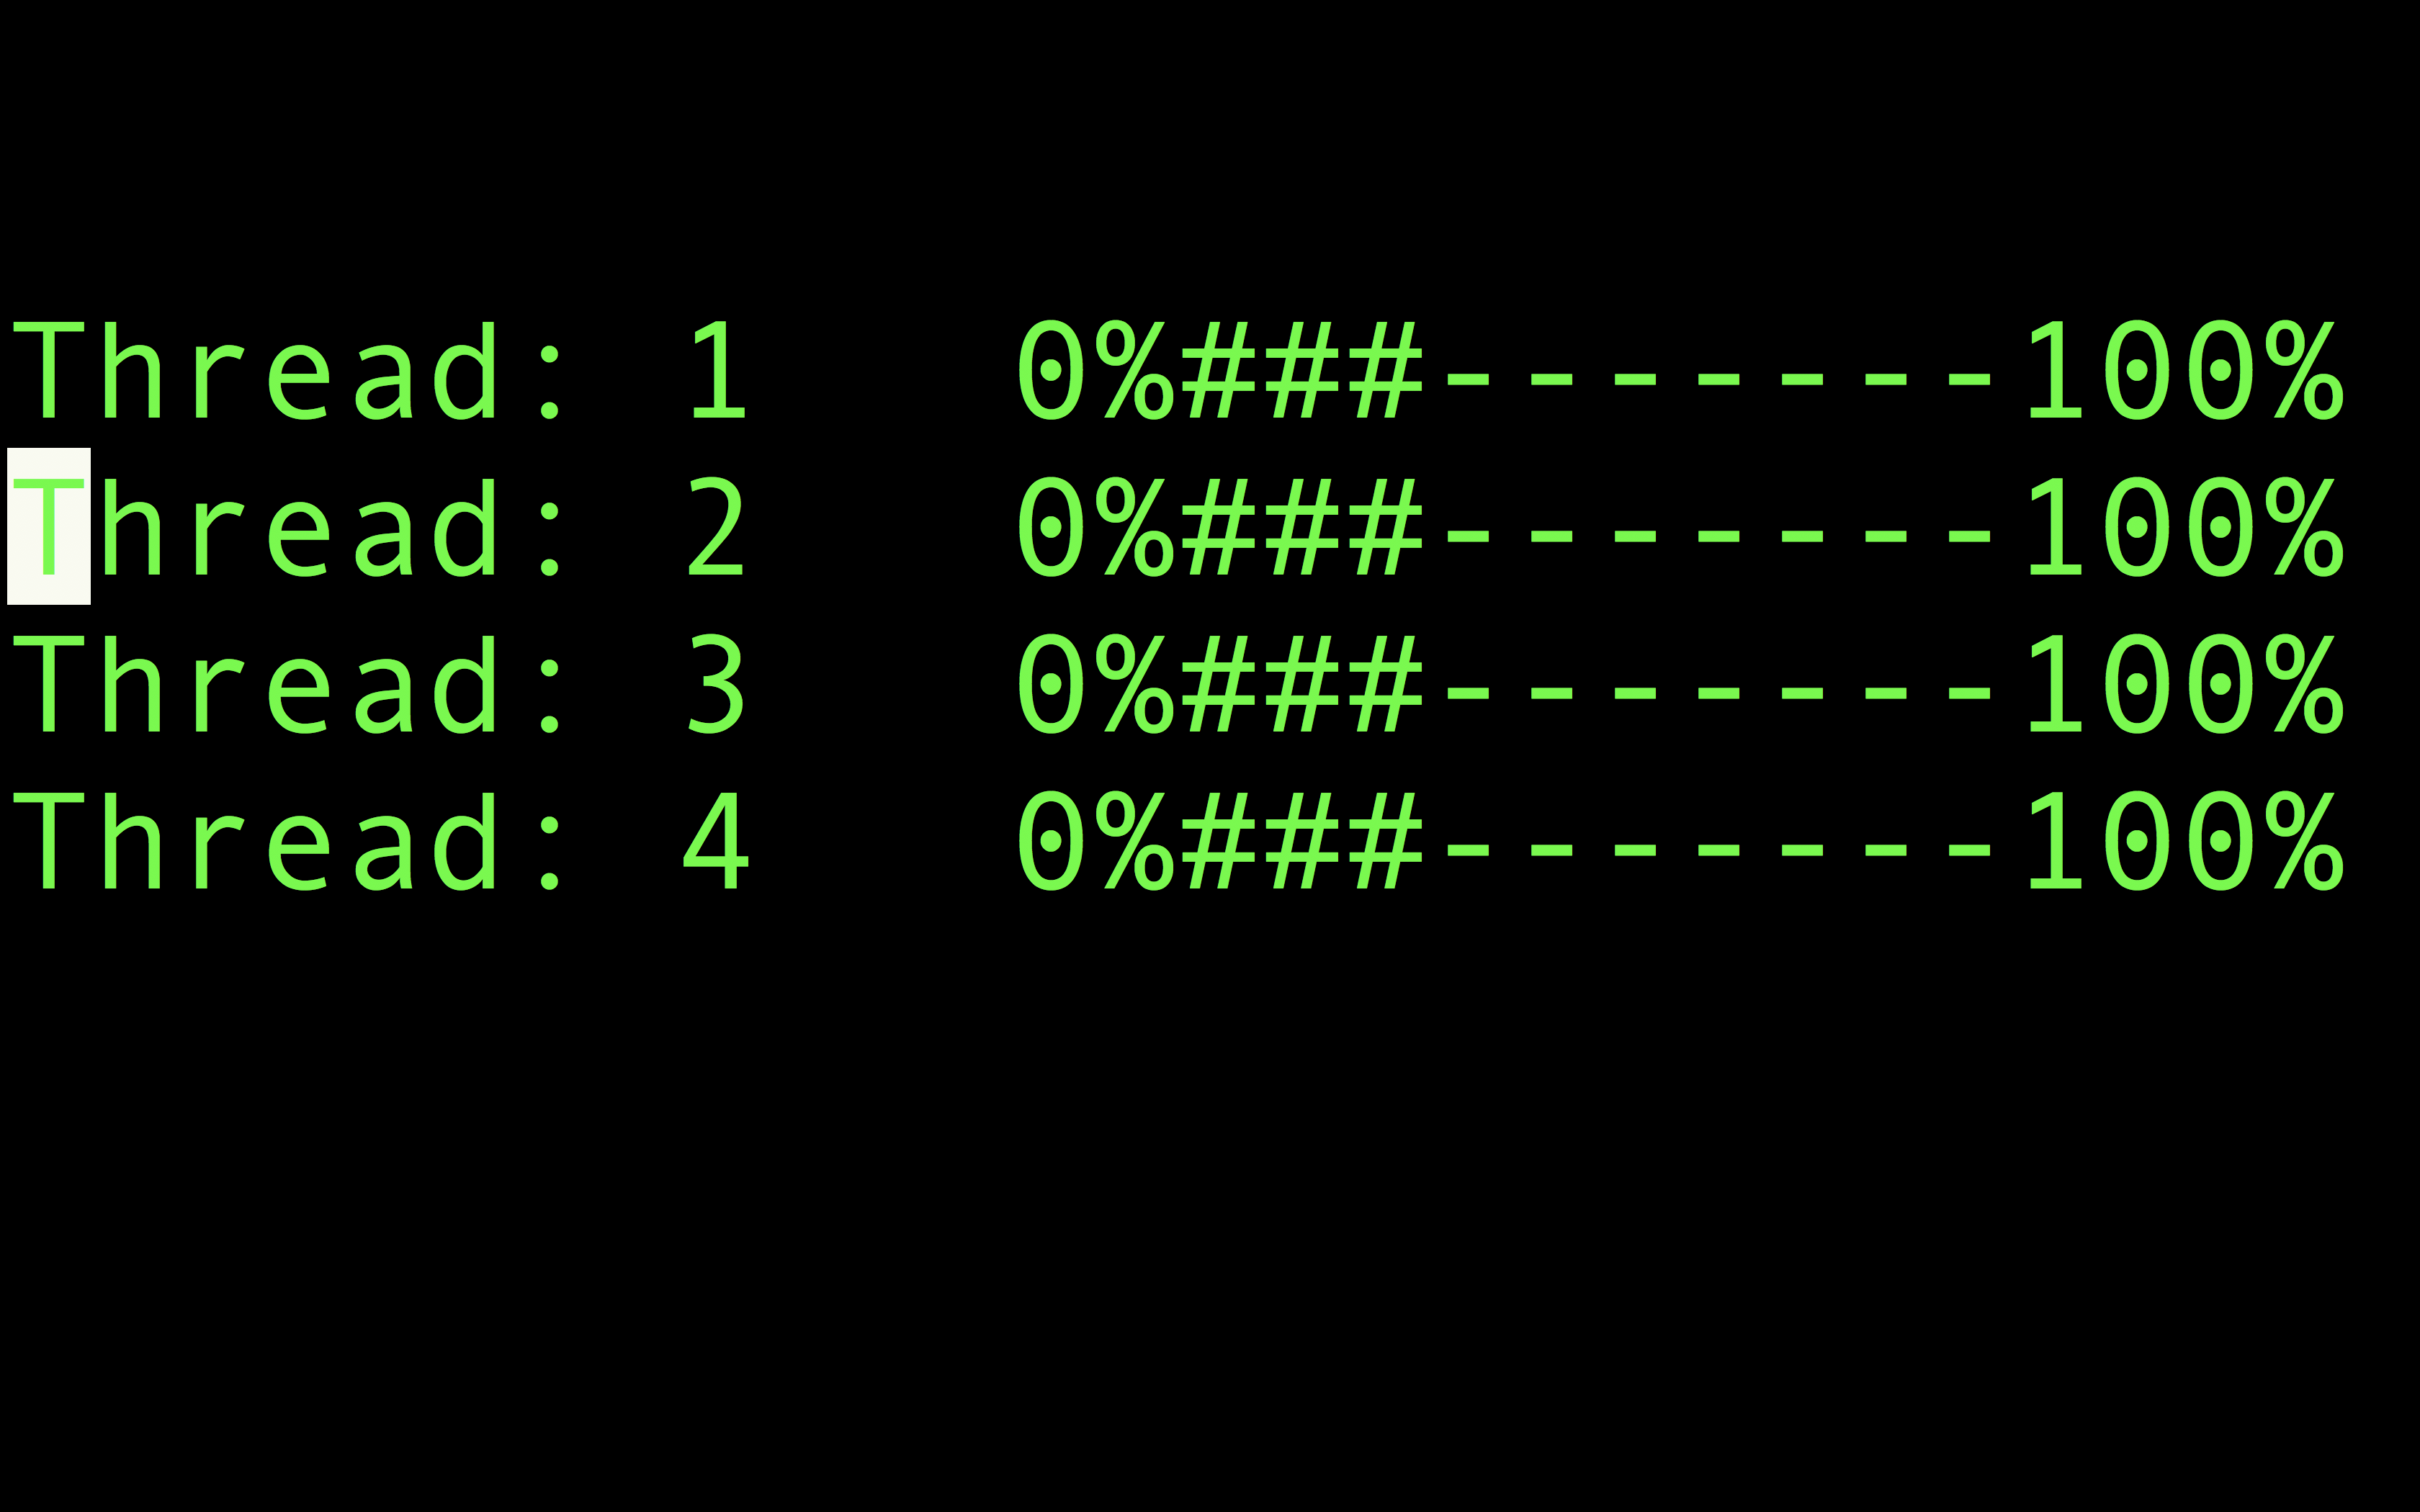
\includegraphics[width=1.11\linewidth]{method/bilder/2}
    \end{subfigure}
    ~ 
    \begin{subfigure}{0.19\textwidth}
        \centering
        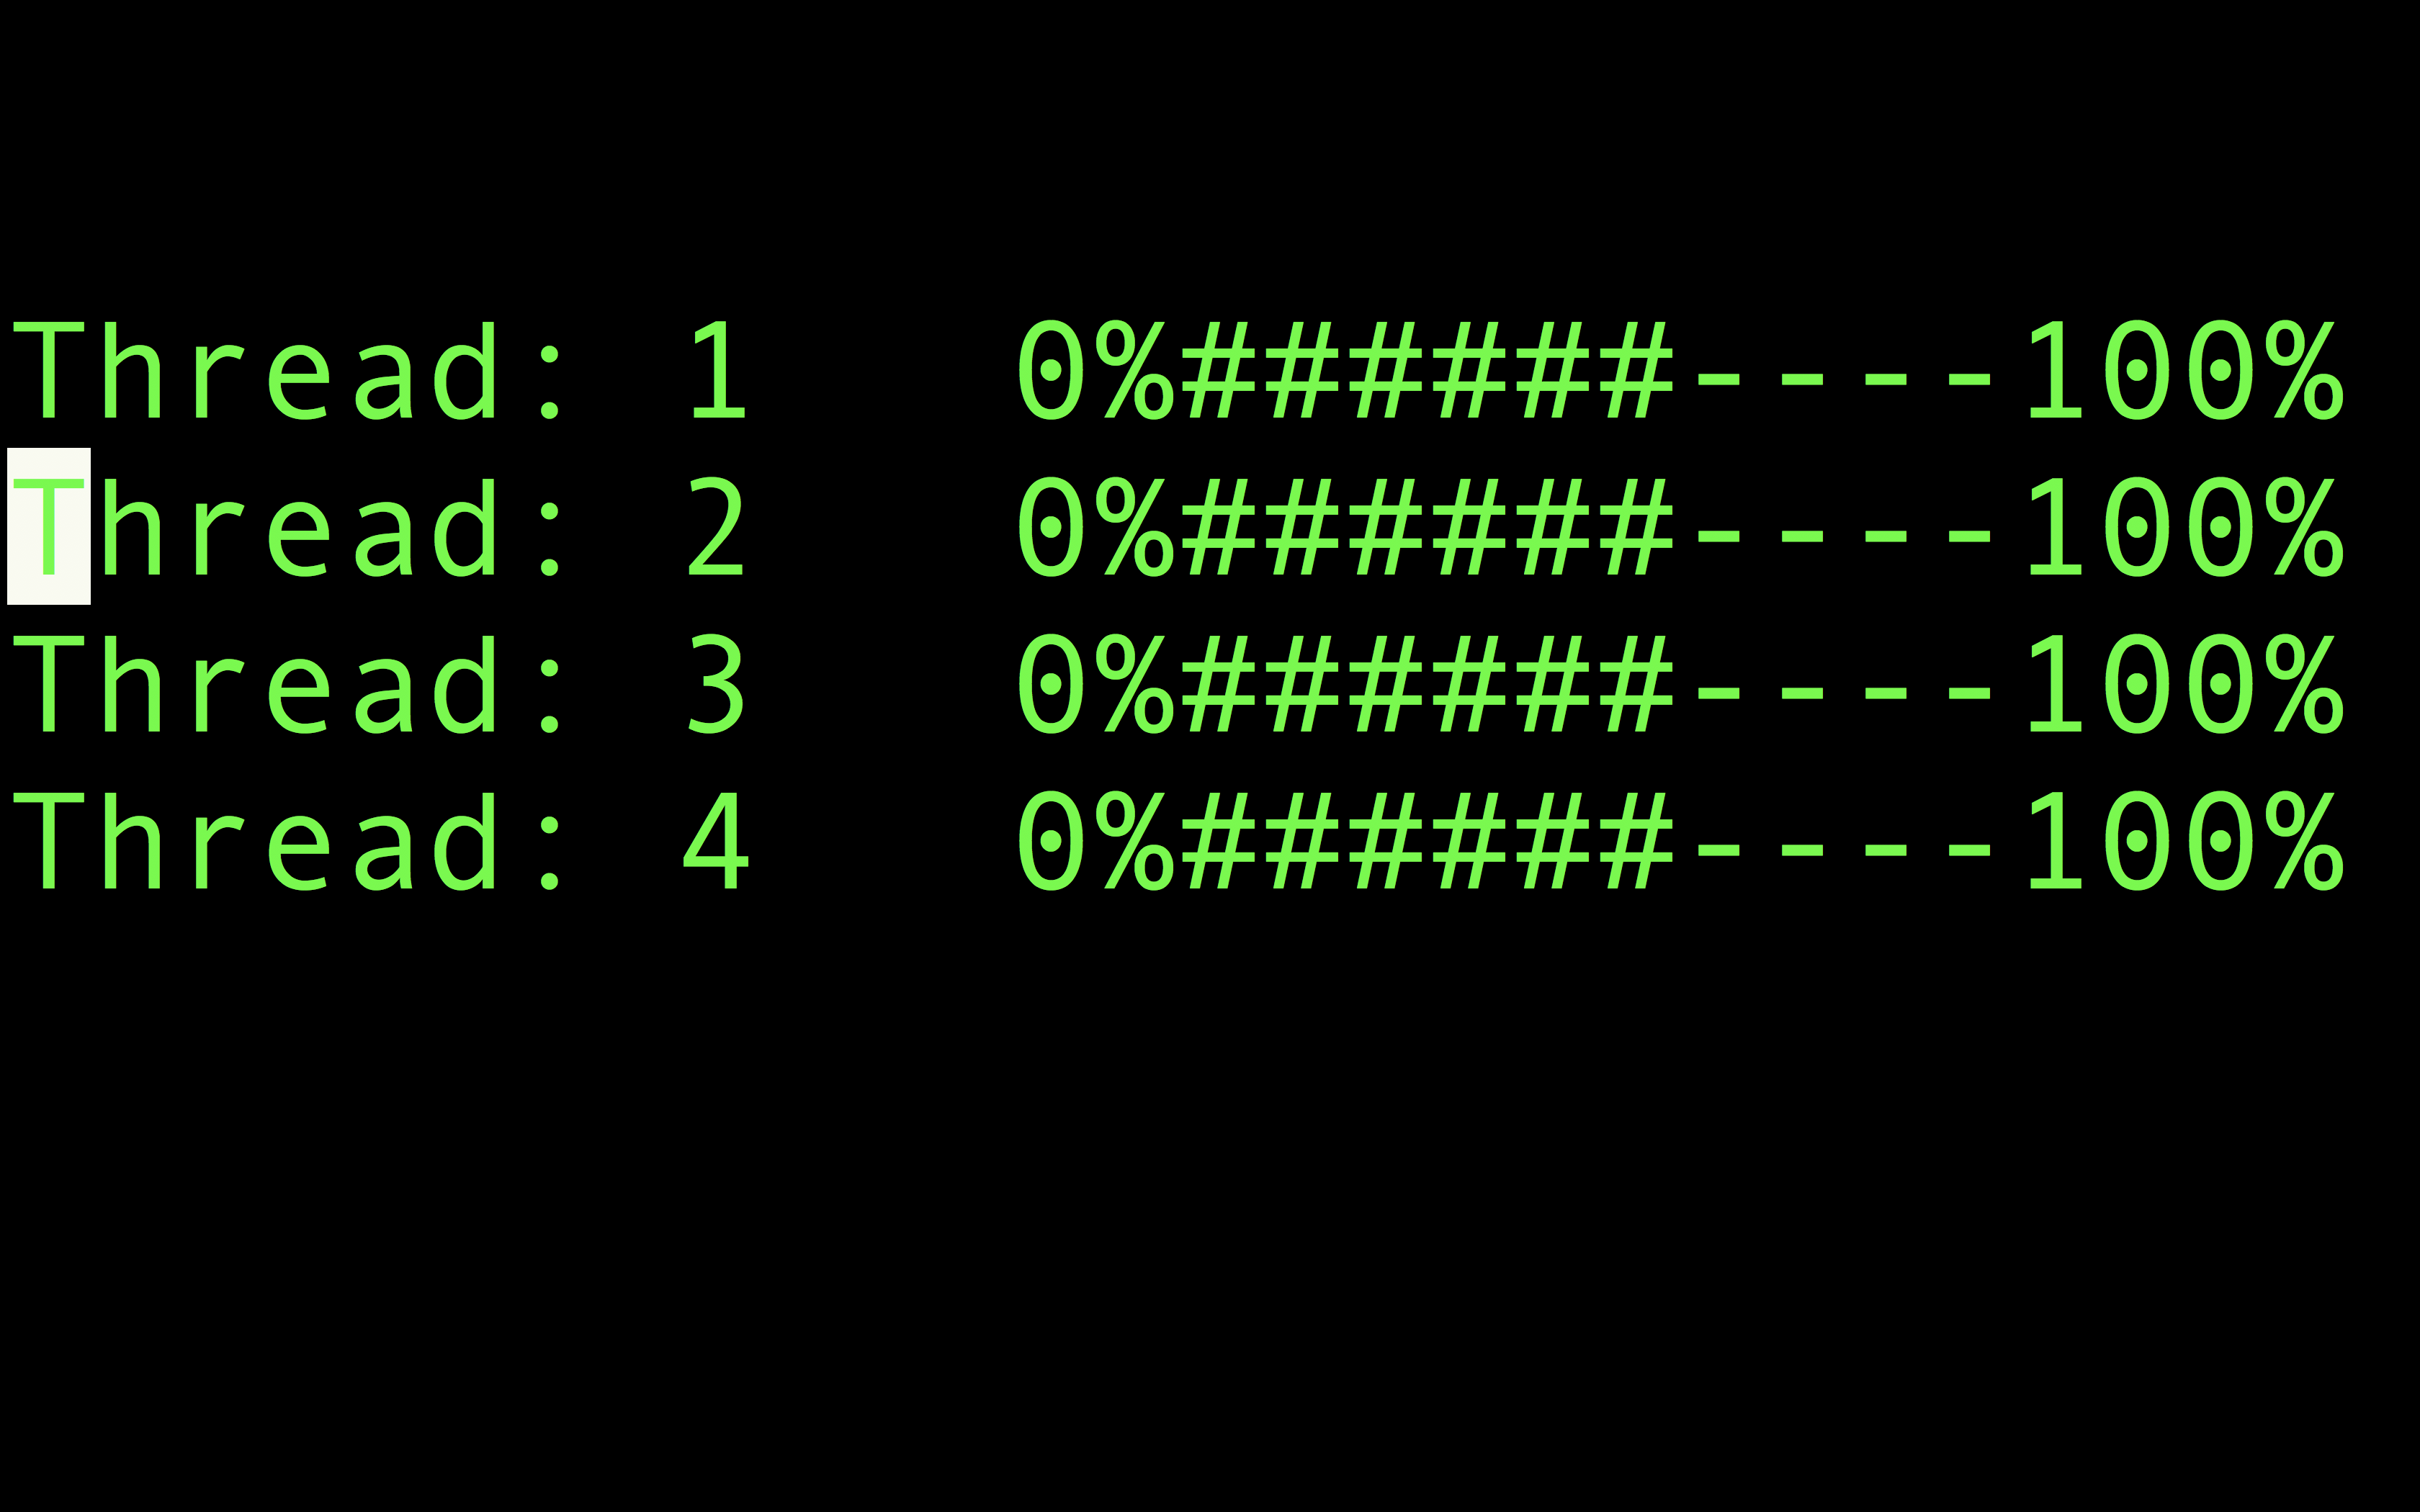
\includegraphics[width=1.11\linewidth]{method/bilder/3}
    \end{subfigure}
    ~ 
    \begin{subfigure}{0.19\textwidth}
        \centering
        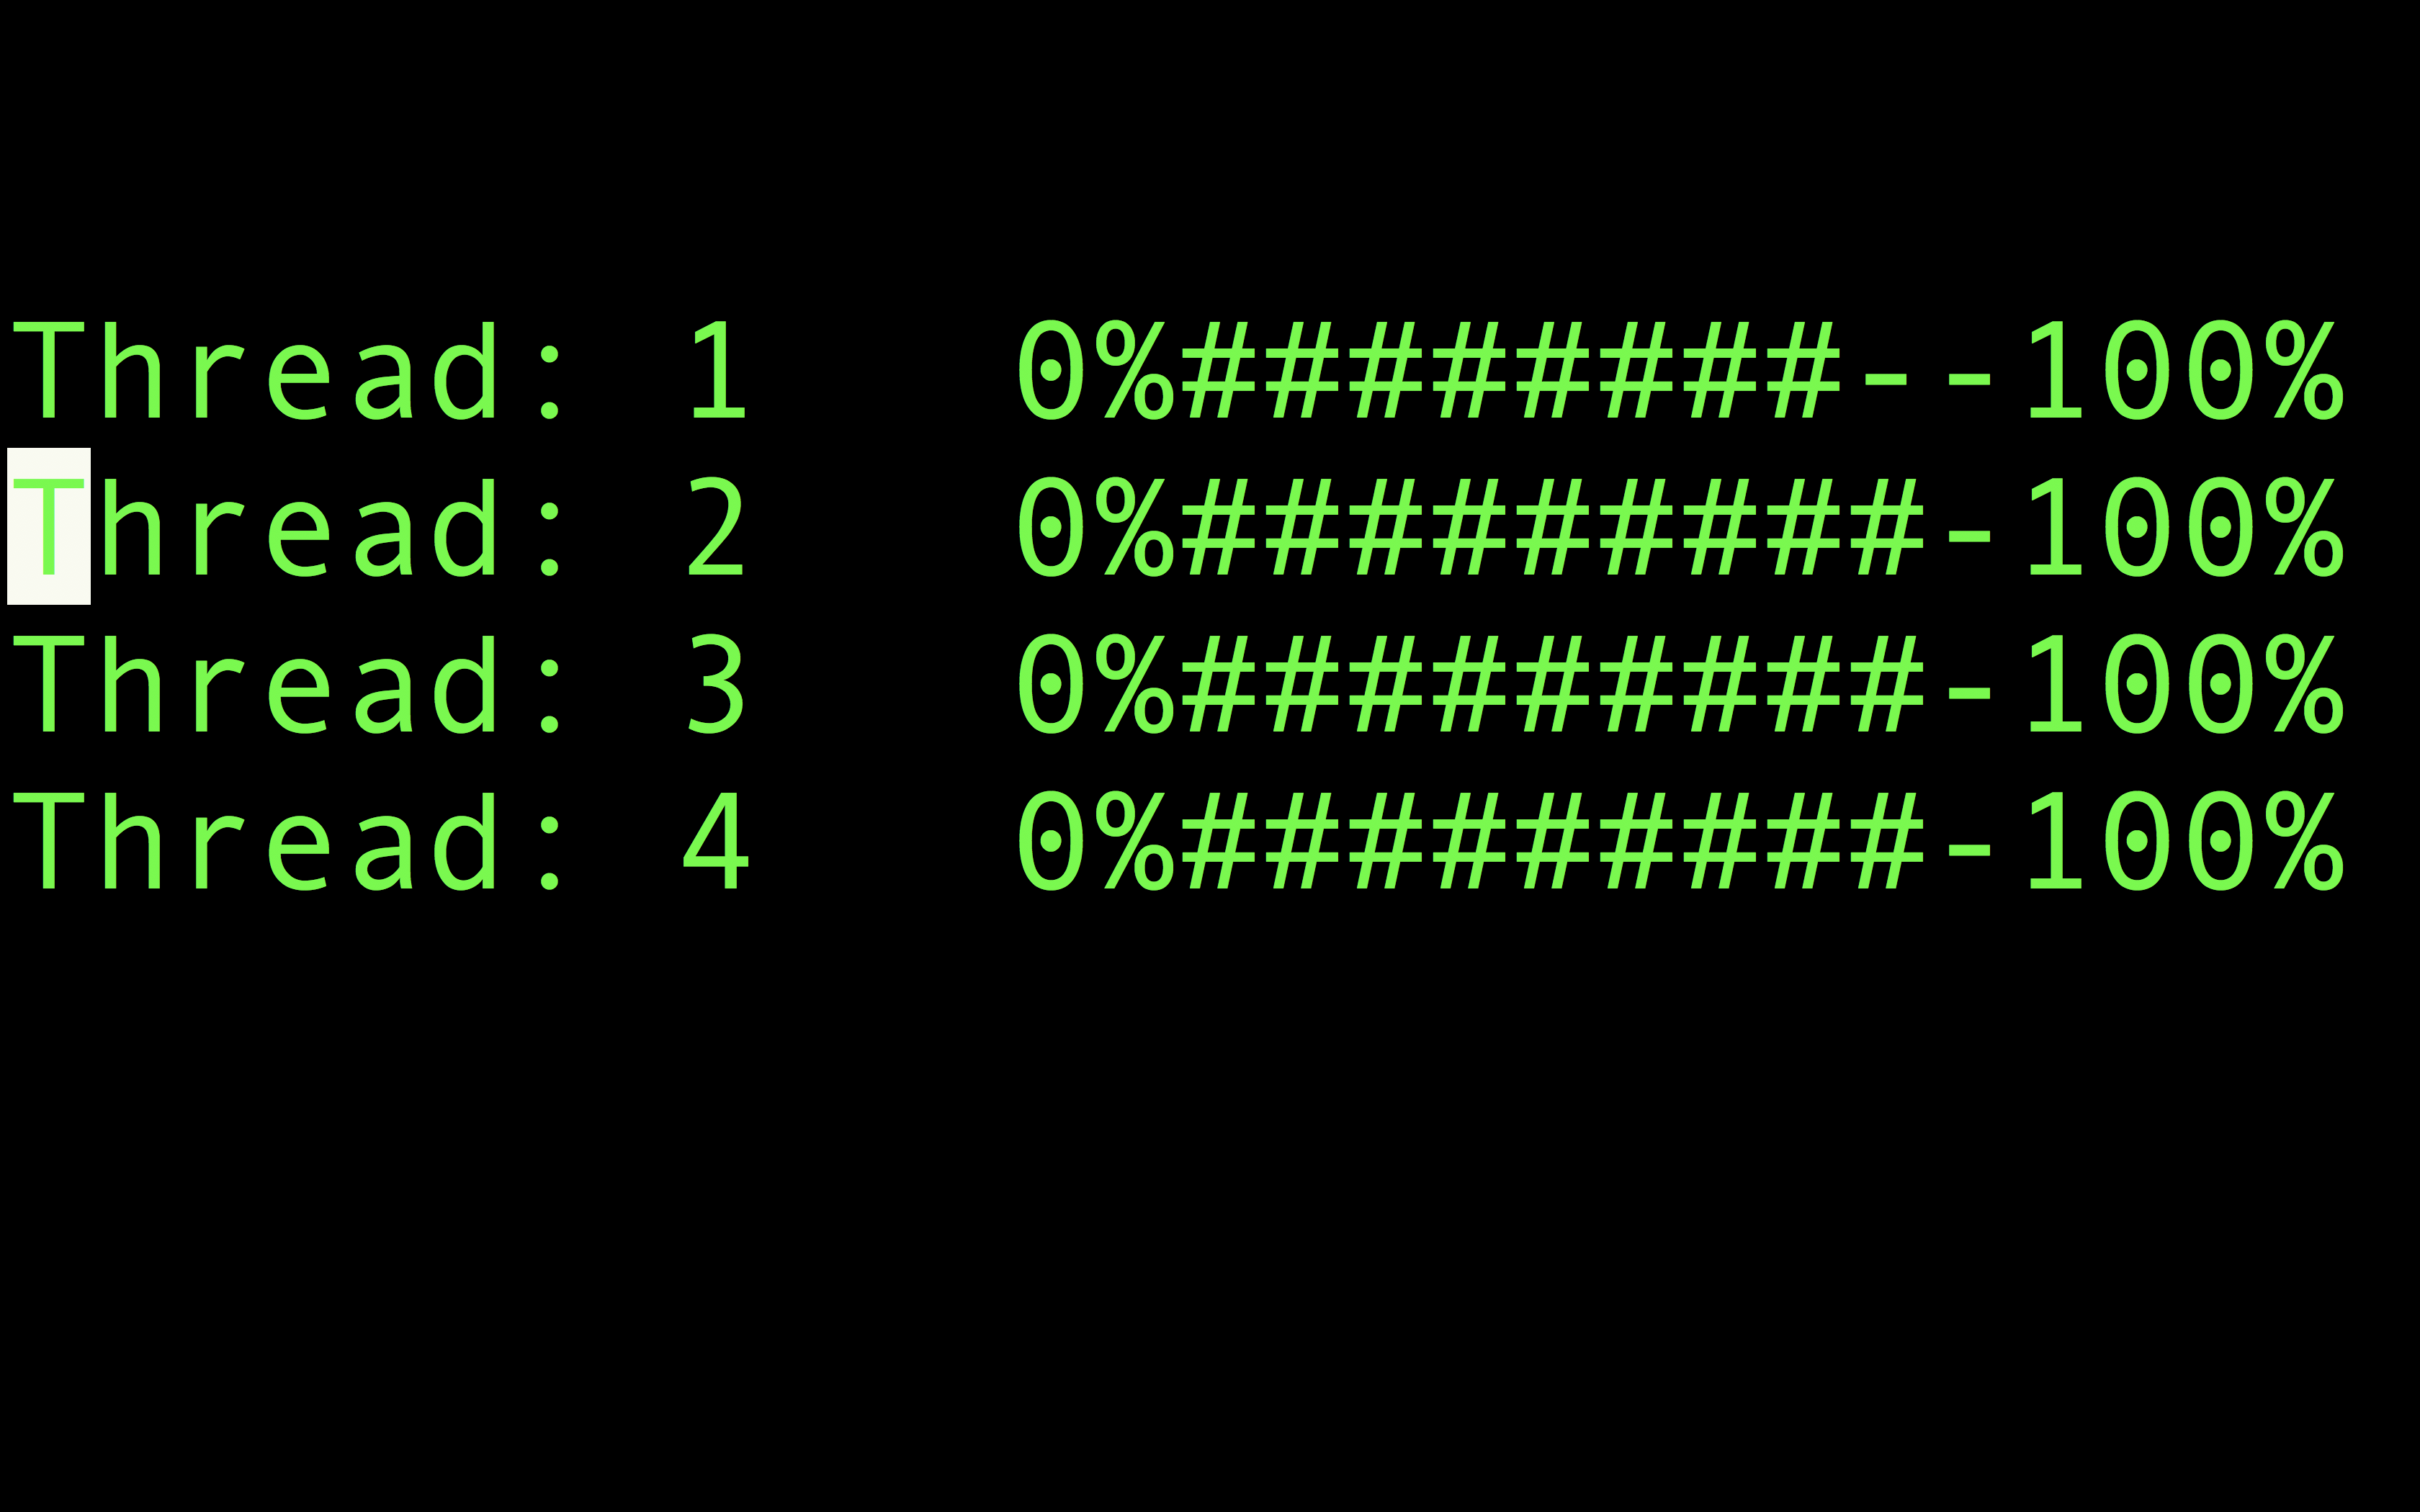
\includegraphics[width=1.11\linewidth]{method/bilder/4}
    \end{subfigure}
    ~ 
    \begin{subfigure}{0.19\textwidth}
        \centering
        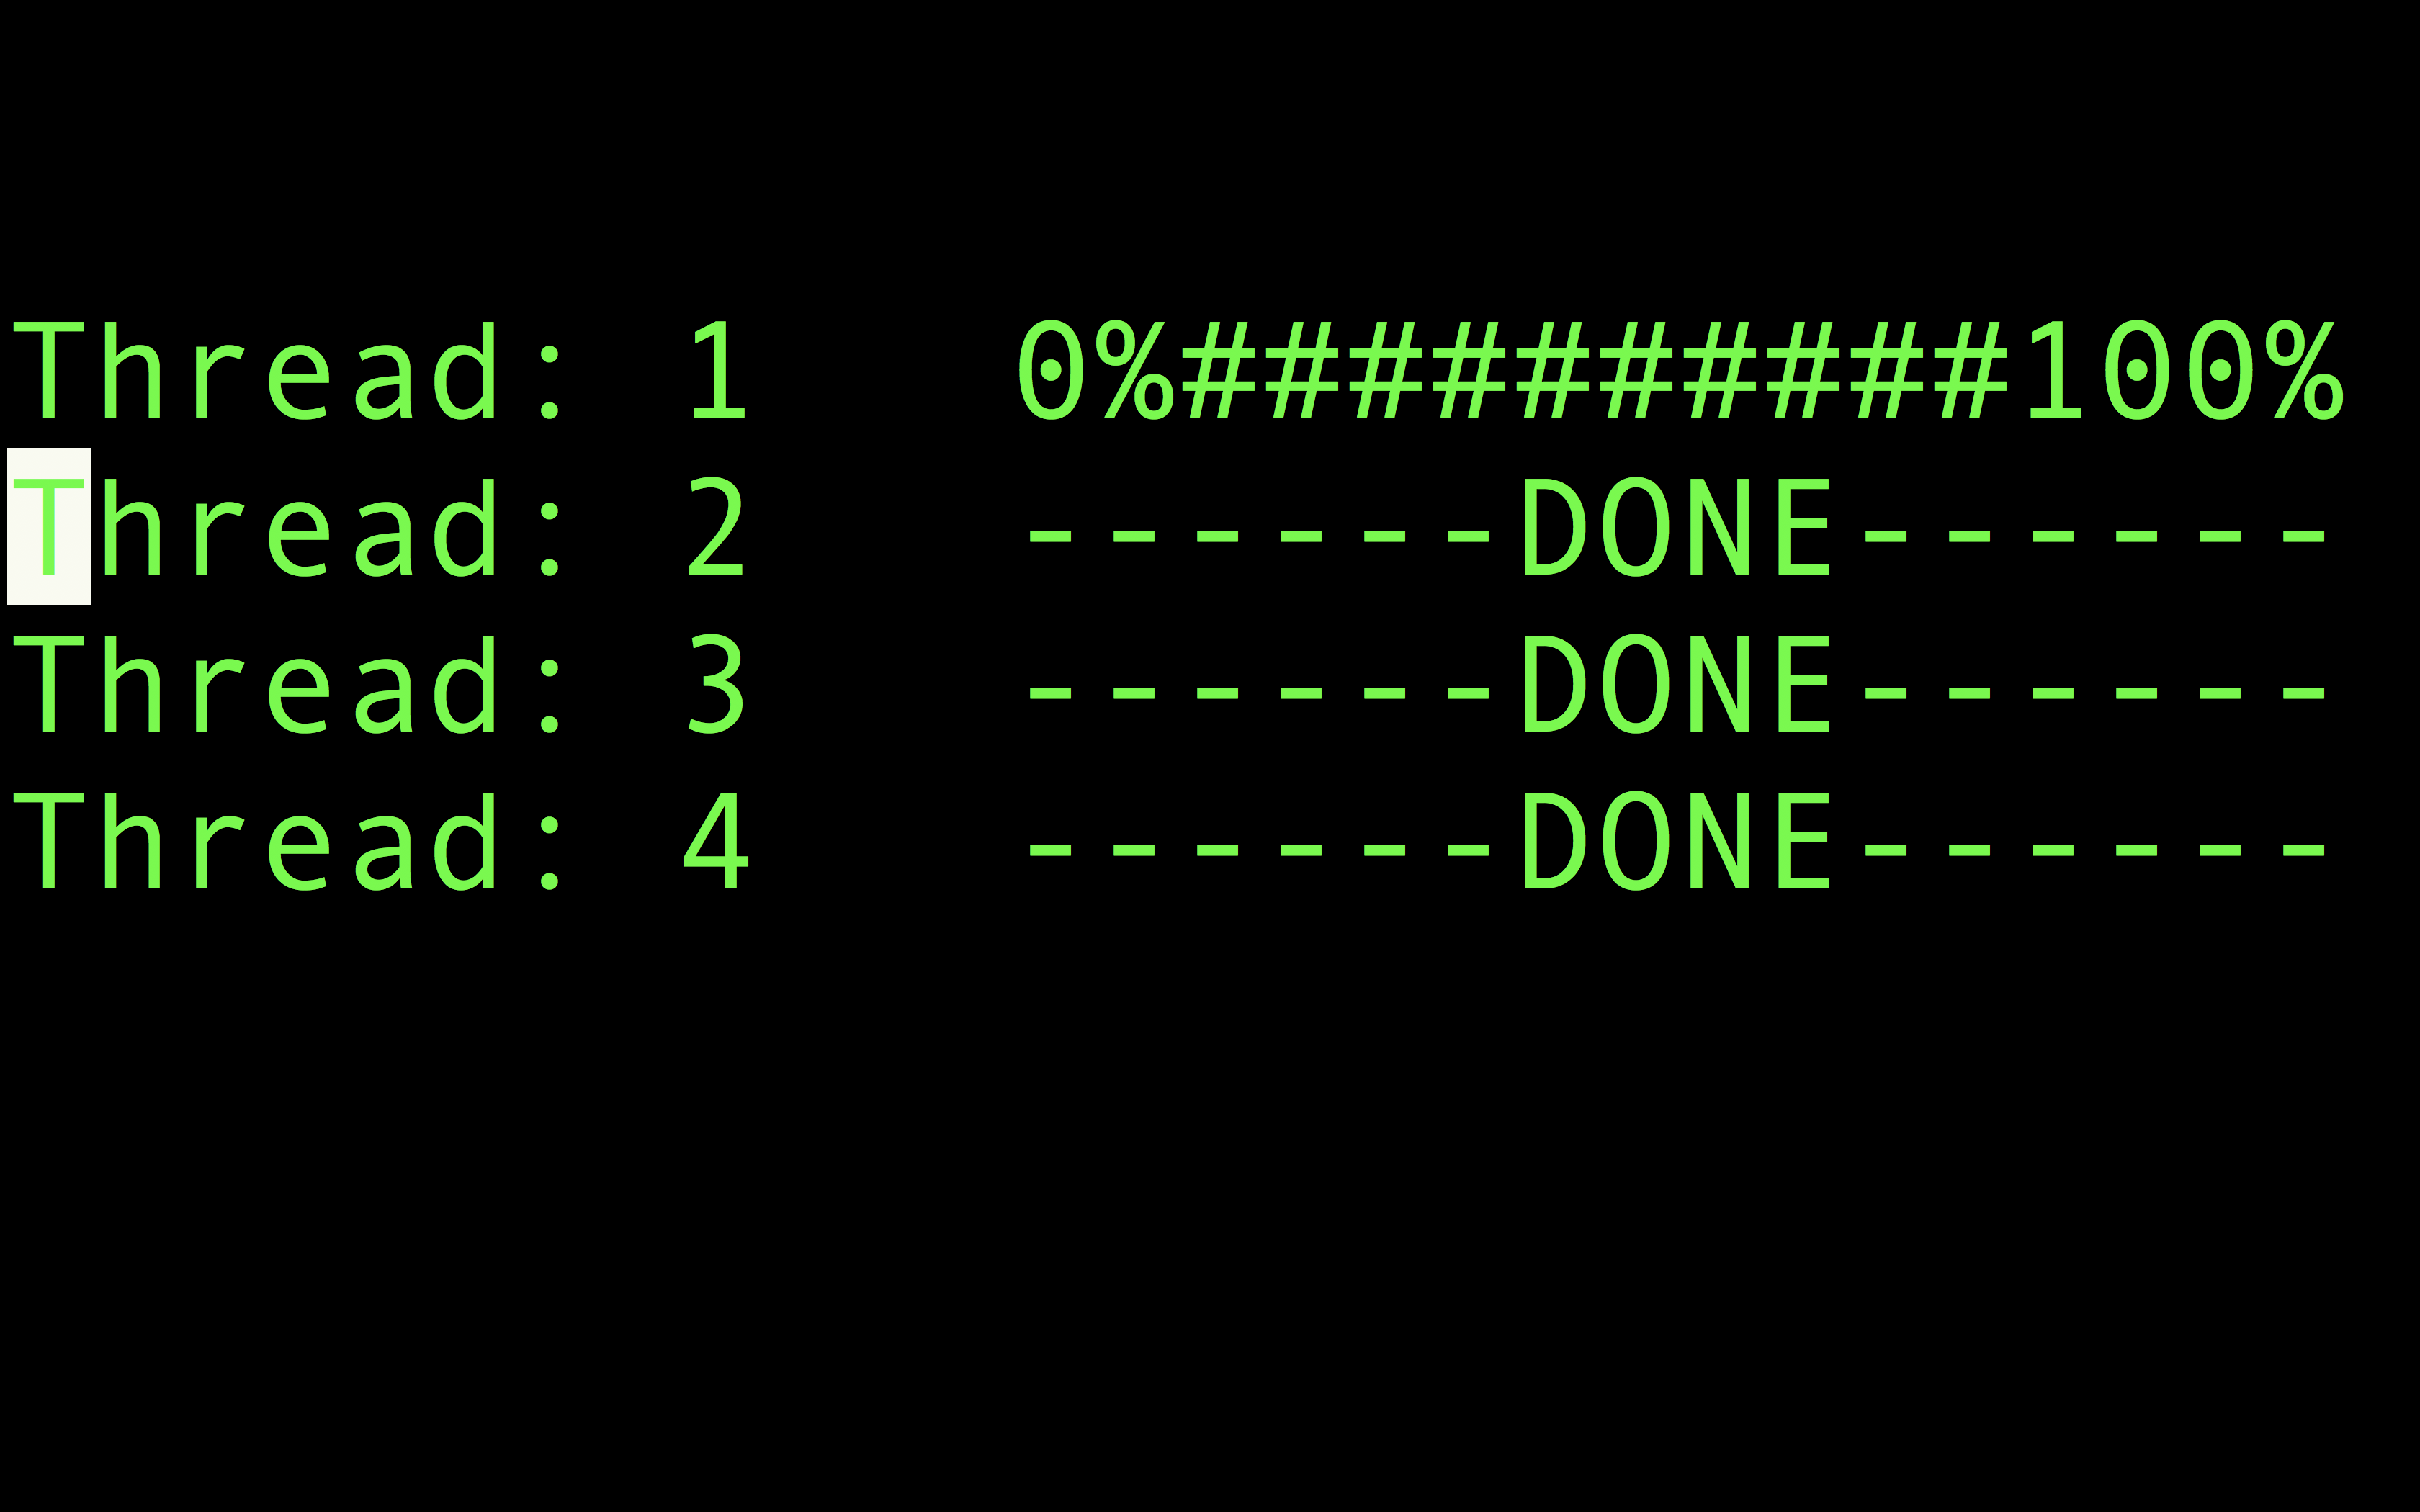
\includegraphics[width=1.11\linewidth]{method/bilder/5}
    \end{subfigure}
    \caption{A progress bar was made for the program. It shows the progress for each individual thread. The progress bar works for 1 to 4 threads. More then 4 threads might look funny. By the way, we are A students in the newly announced PRO101 subject. }
    \label{fig:progress}
\end{figure}


\footnote{
    \href
    {https://shortridgedailyecho.org/wp-content/uploads/2017/08/definition-procrastination.png}
    {
    \color{blue}{PRO101: Procrastination for students}
    }
    }
% \animategraphics{12}{gif-}{1}{32}



\section{Result \& Discussion}
\pagebreak
\subsection{5a \& 5b}
\begin{figure}[H]
    \centering
    \begin{subfigure}{0.5\textwidth}
        \centering
        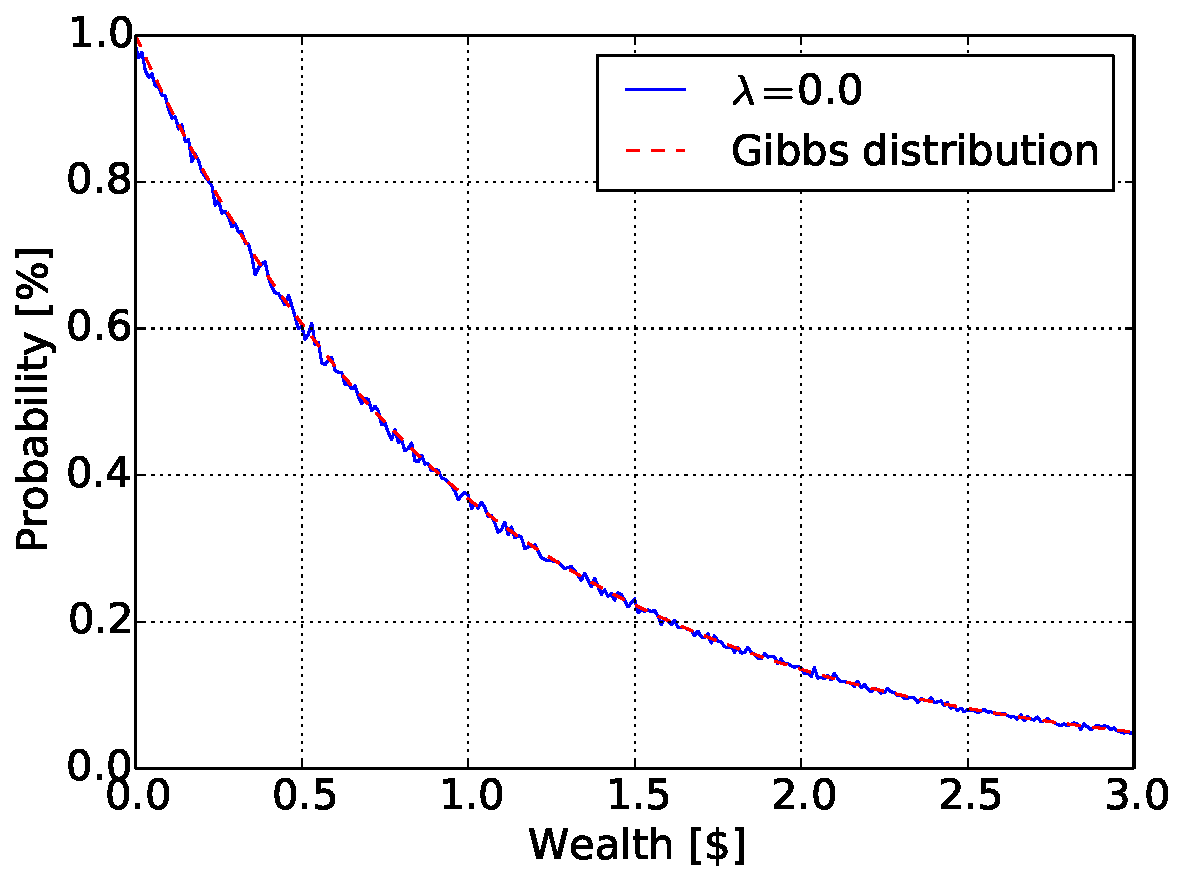
\includegraphics[width=\linewidth]{result/bilder/5a-correct}
        \caption{}
    \end{subfigure}%
    ~ 
    \begin{subfigure}{0.5\textwidth}
        \centering
        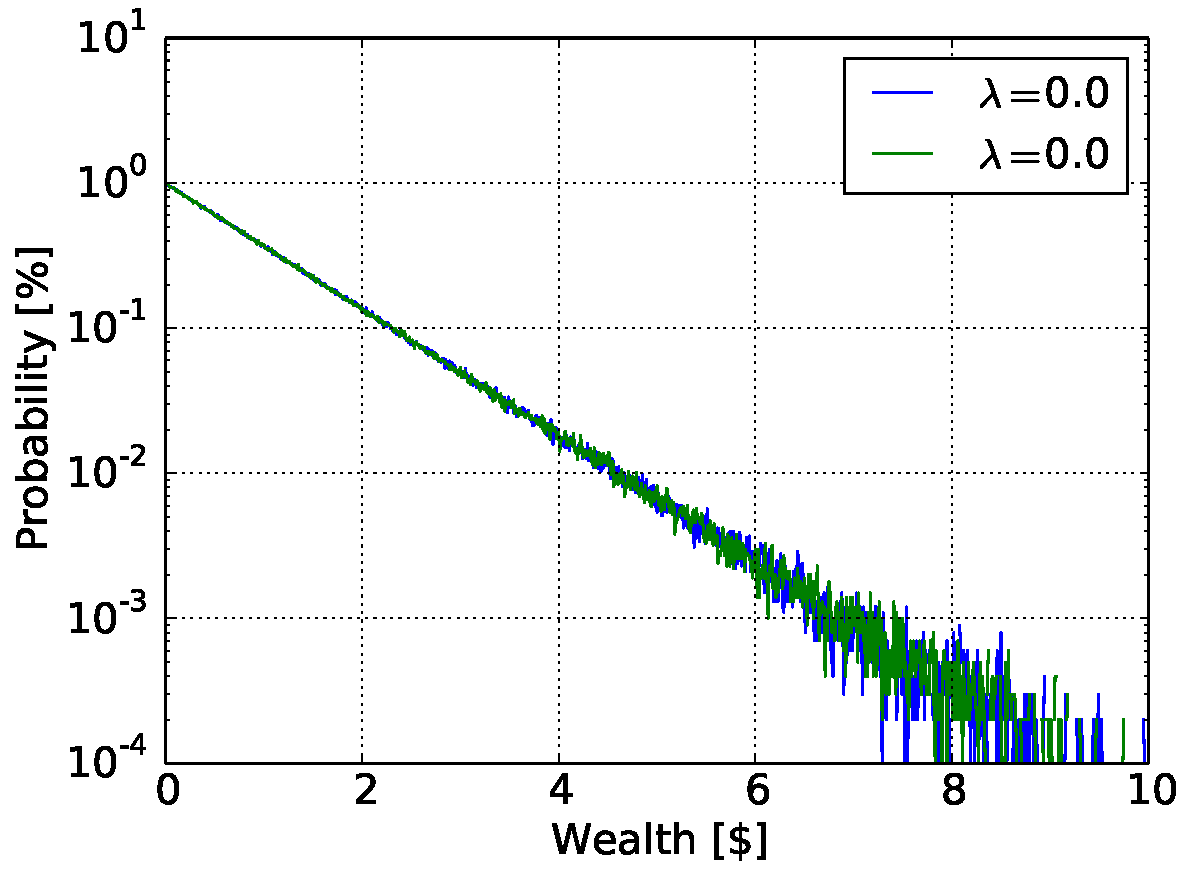
\includegraphics[width=\linewidth]{result/bilder/5b-correct}
        \caption{}
    \end{subfigure}
    \caption{a) Shows how E behaves around $T_C$ b) Shows how |M| develops near $T_C$.}
    \label{fig:5a-b}
\end{figure}




























\pagebreak
\subsection{5c}
\begin{figure}[H]
    \centering
    \begin{subfigure}{0.5\textwidth}
        \centering
        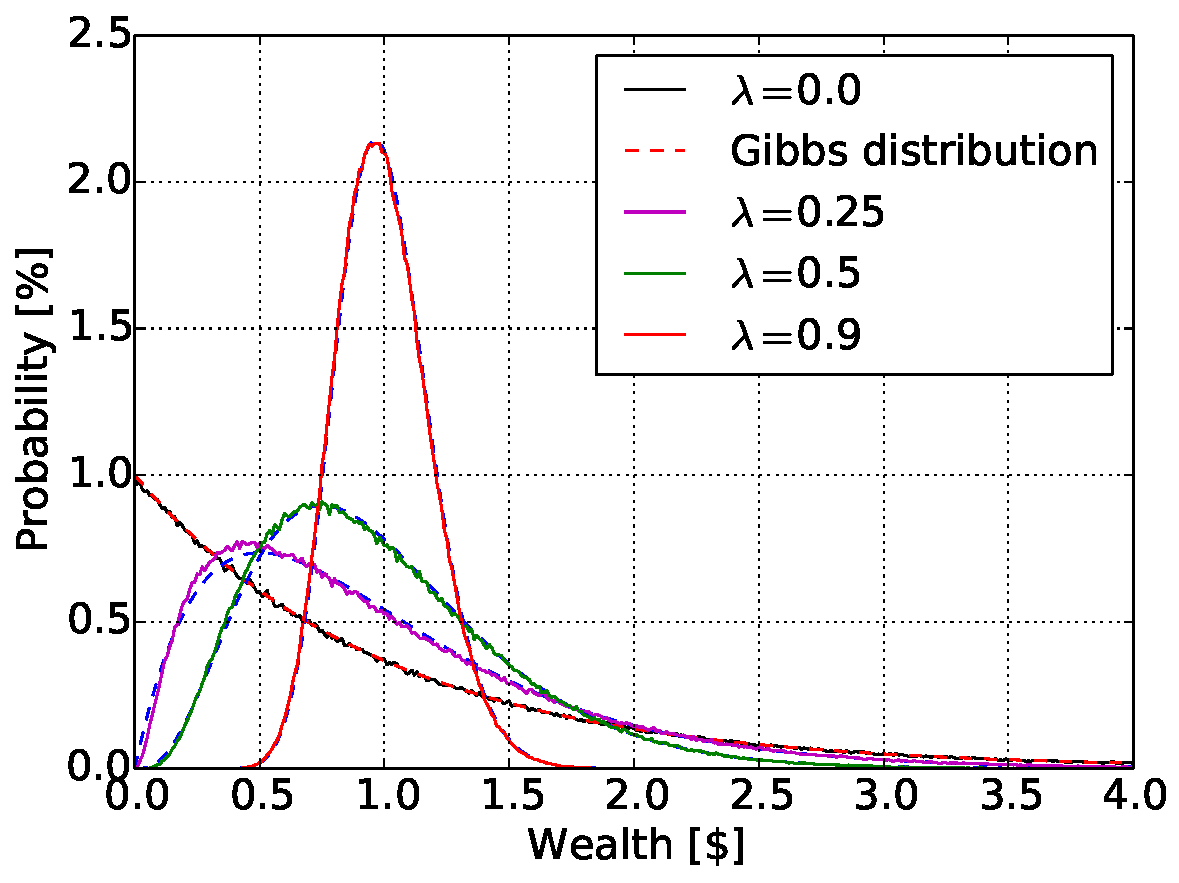
\includegraphics[width=\linewidth]{result/bilder/5c}
        \caption{}
    \end{subfigure}%
    ~ 
    \begin{subfigure}{0.5\textwidth}
        \centering
        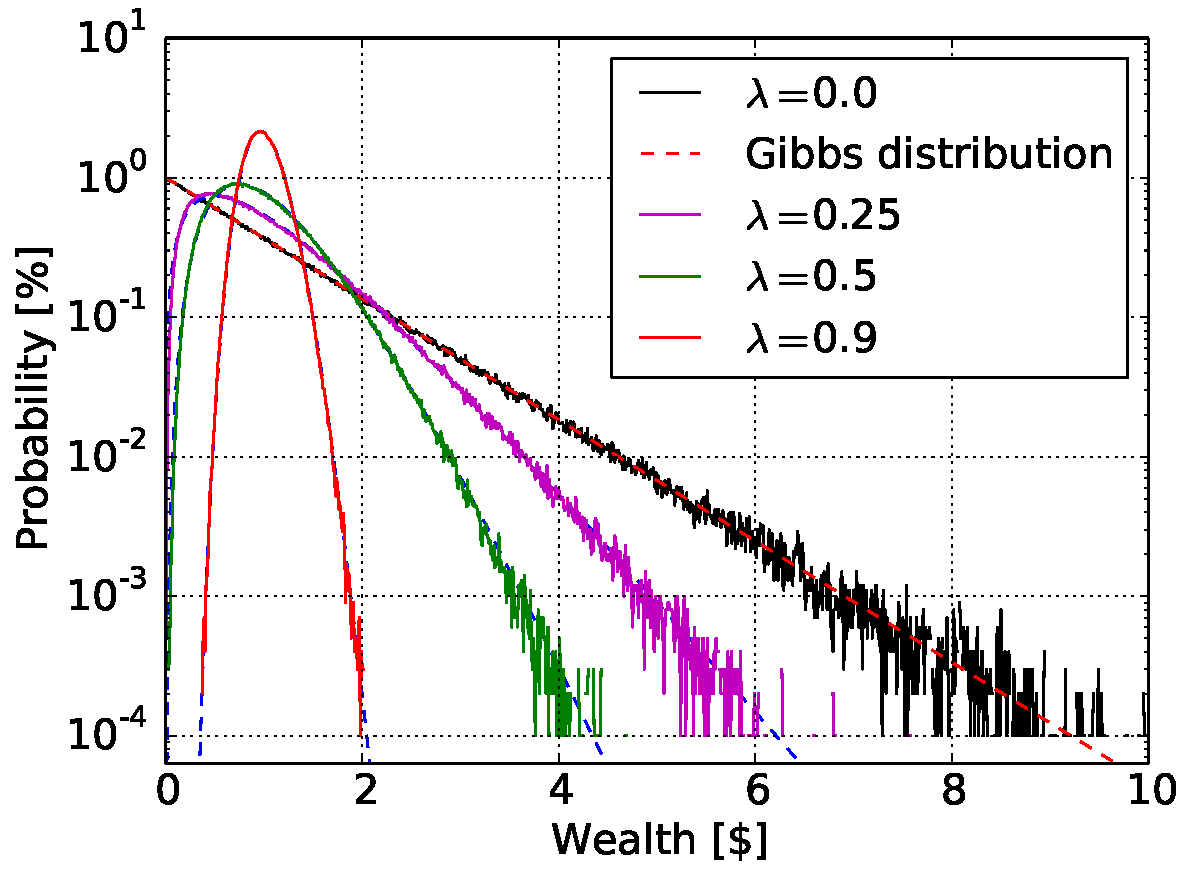
\includegraphics[width=\linewidth]{result/bilder/5c-log}
        \caption{}
    \end{subfigure}
    \caption{a) Shows how E behaves around $T_C$ b) Shows how |M| develops near $T_C$.}
    \label{fig:5c}
\end{figure}




























\pagebreak
\subsection{5d}
\begin{figure}[H]
    \centering
    \begin{subfigure}{0.5\textwidth}
        \centering
        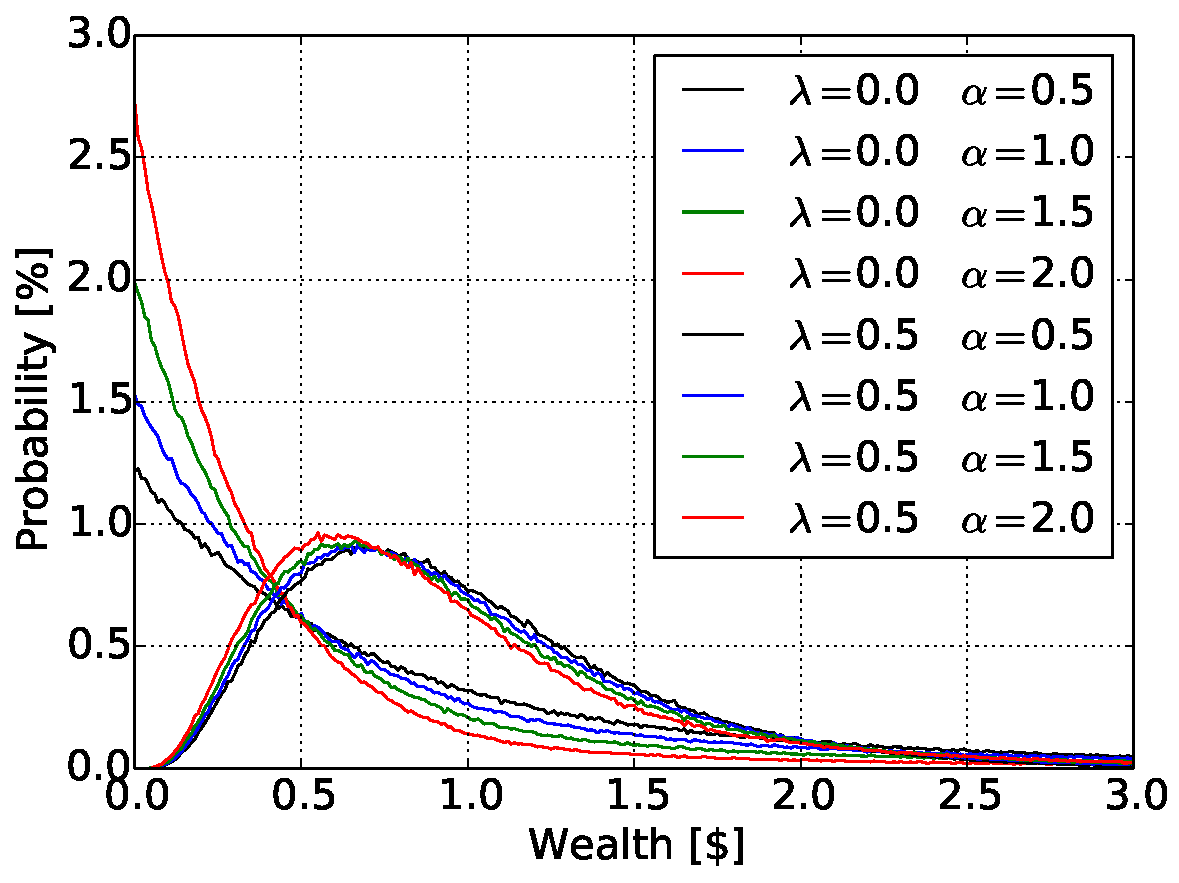
\includegraphics[width=\linewidth]{result/bilder/5d-0050}
        \caption{}
    \end{subfigure}%
    ~ 
    \begin{subfigure}{0.5\textwidth}
        \centering
        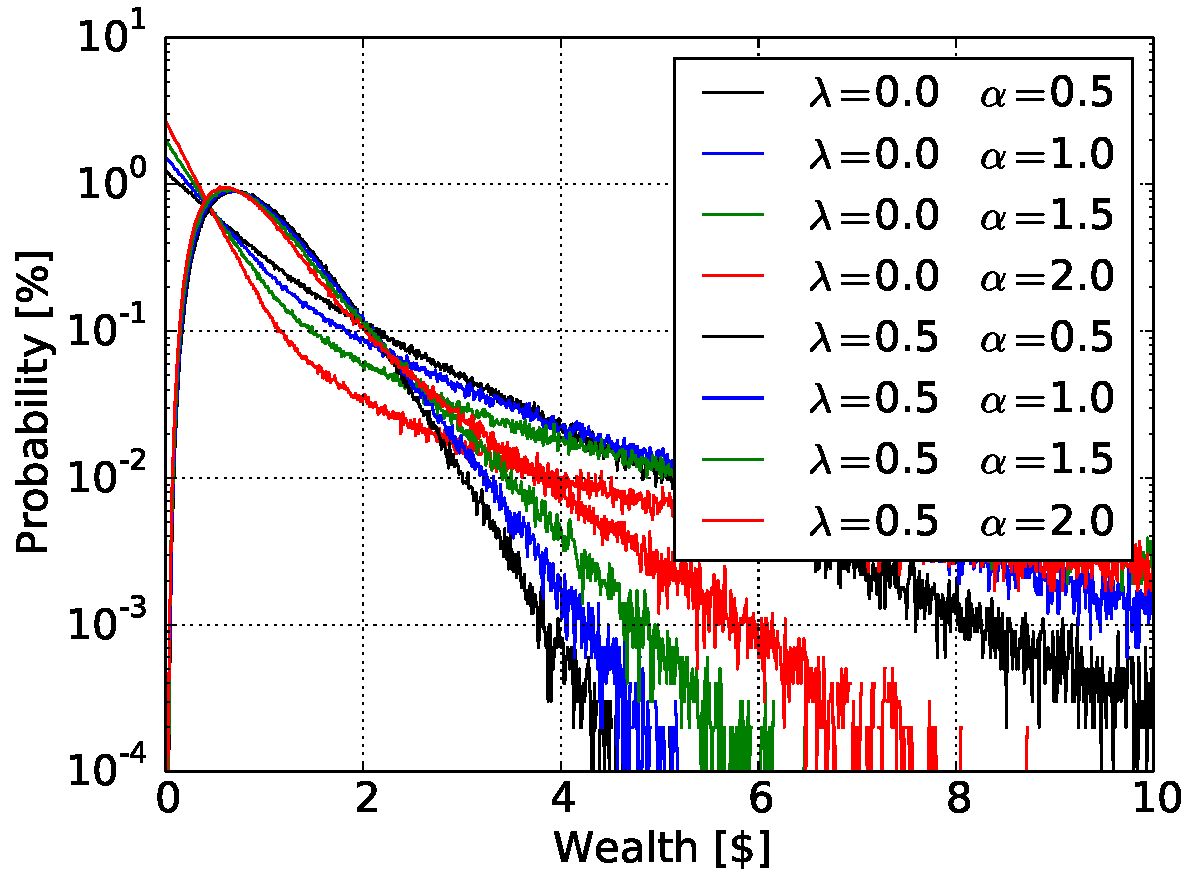
\includegraphics[width=\linewidth]{result/bilder/5d-0050-log}
        \caption{}
    \end{subfigure}
    \caption{a) Shows how E behaves around $T_C$ b) Shows how |M| develops near $T_C$.}
    \label{fig:5d-0050}
\end{figure}



\begin{figure}[H]
    \centering
    \begin{subfigure}{0.5\textwidth}
        \centering
        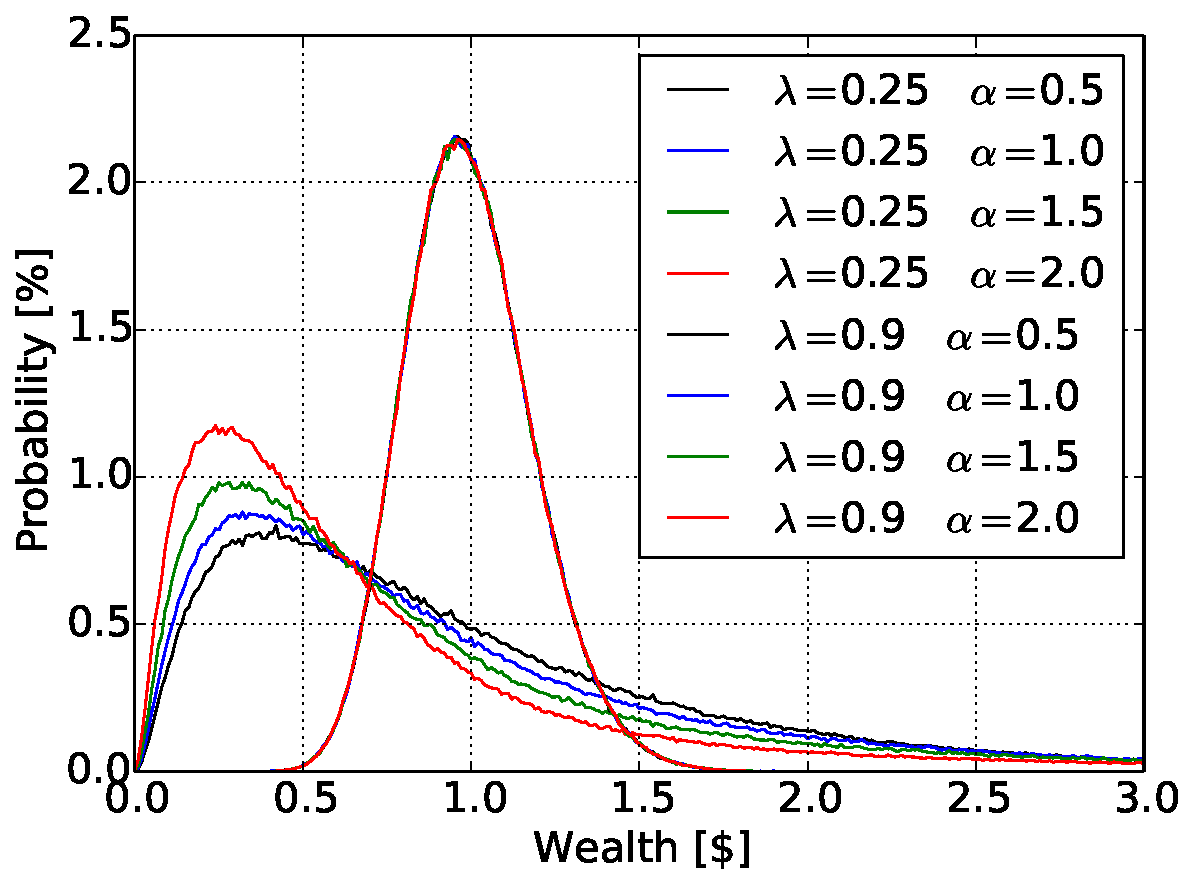
\includegraphics[width=\linewidth]{result/bilder/5d-2590}
        \caption{}
    \end{subfigure}%
    ~ 
    \begin{subfigure}{0.5\textwidth}
        \centering
        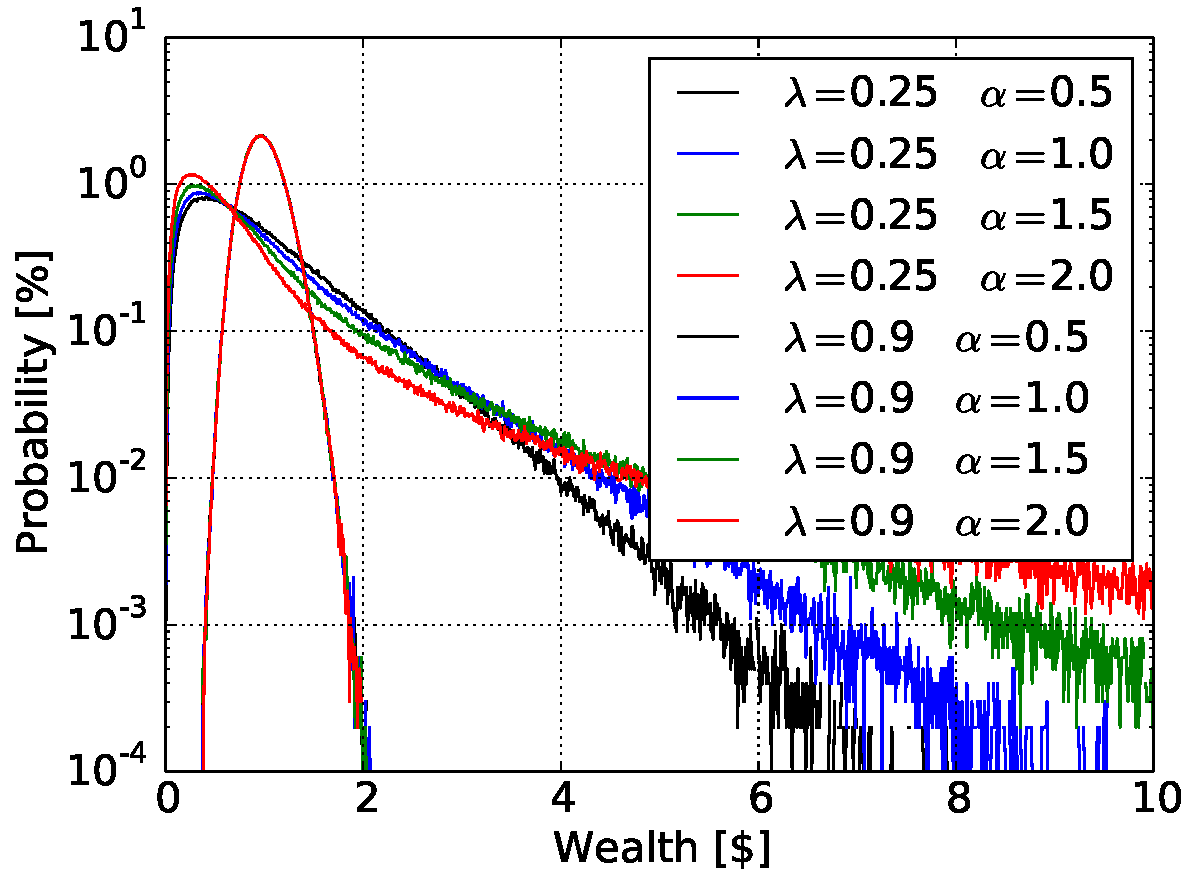
\includegraphics[width=\linewidth]{result/bilder/5d-2590-log}
        \caption{}
    \end{subfigure}
    \caption{a) Shows how E behaves around $T_C$ b) Shows how |M| develops near $T_C$.}
    \label{fig:5d-2590}
\end{figure}



\begin{figure}[H]
    \centering
    \begin{subfigure}{0.5\textwidth}
        \centering
        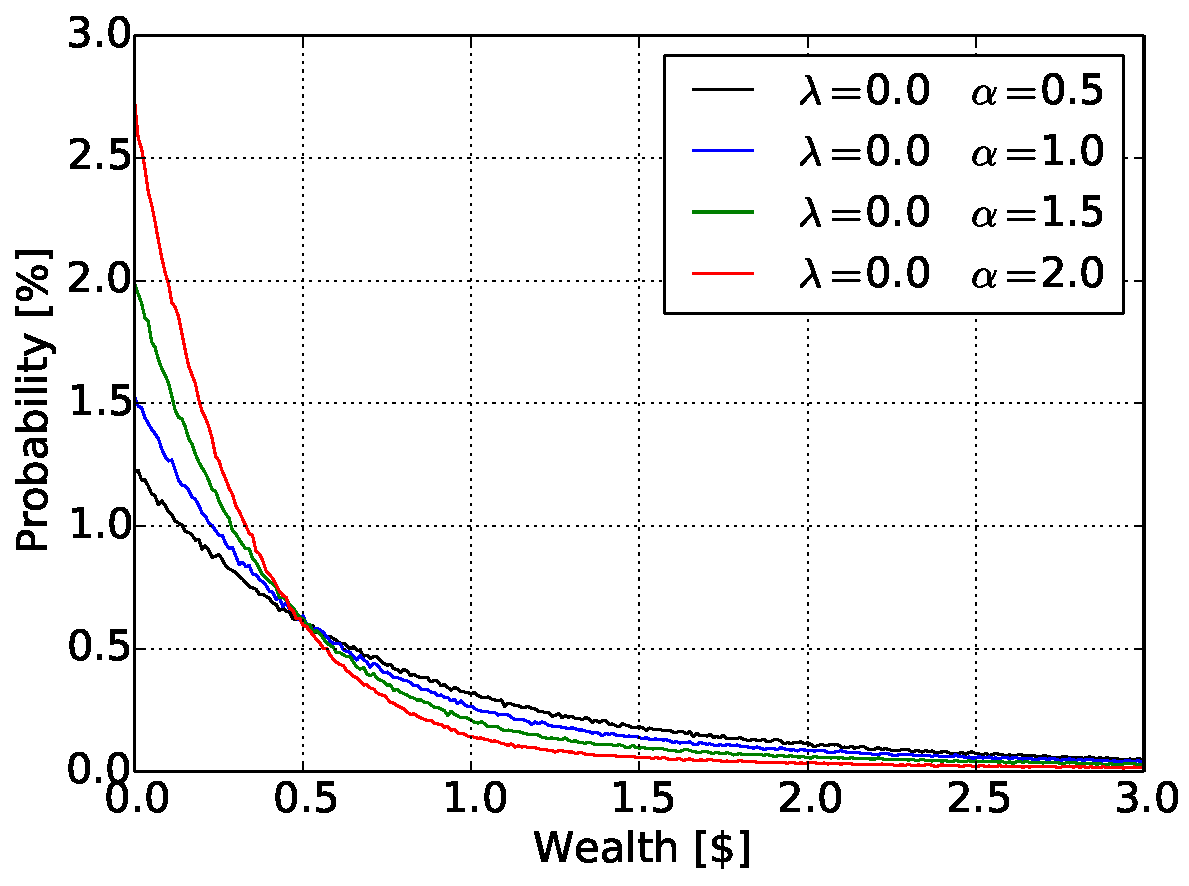
\includegraphics[width=\linewidth]{result/bilder/5d-00}
        \caption{}
    \end{subfigure}%
    ~ 
    \begin{subfigure}{0.5\textwidth}
        \centering
        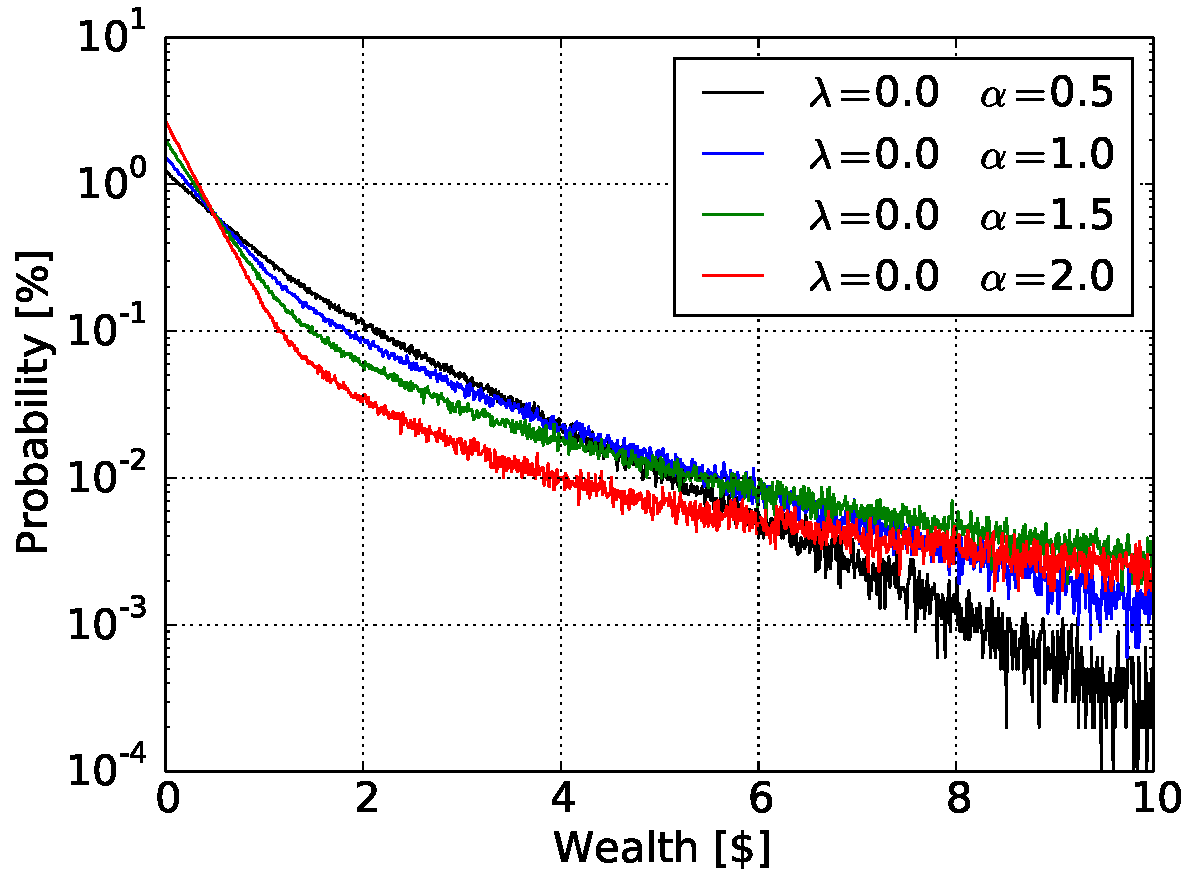
\includegraphics[width=\linewidth]{result/bilder/5d-00-log}
        \caption{}
    \end{subfigure}
    \caption{a) Shows how E behaves around $T_C$ b) Shows how |M| develops near $T_C$.}
    \label{fig:5d-00}
\end{figure}



\begin{figure}[H]
    \centering
    \begin{subfigure}{0.5\textwidth}
        \centering
        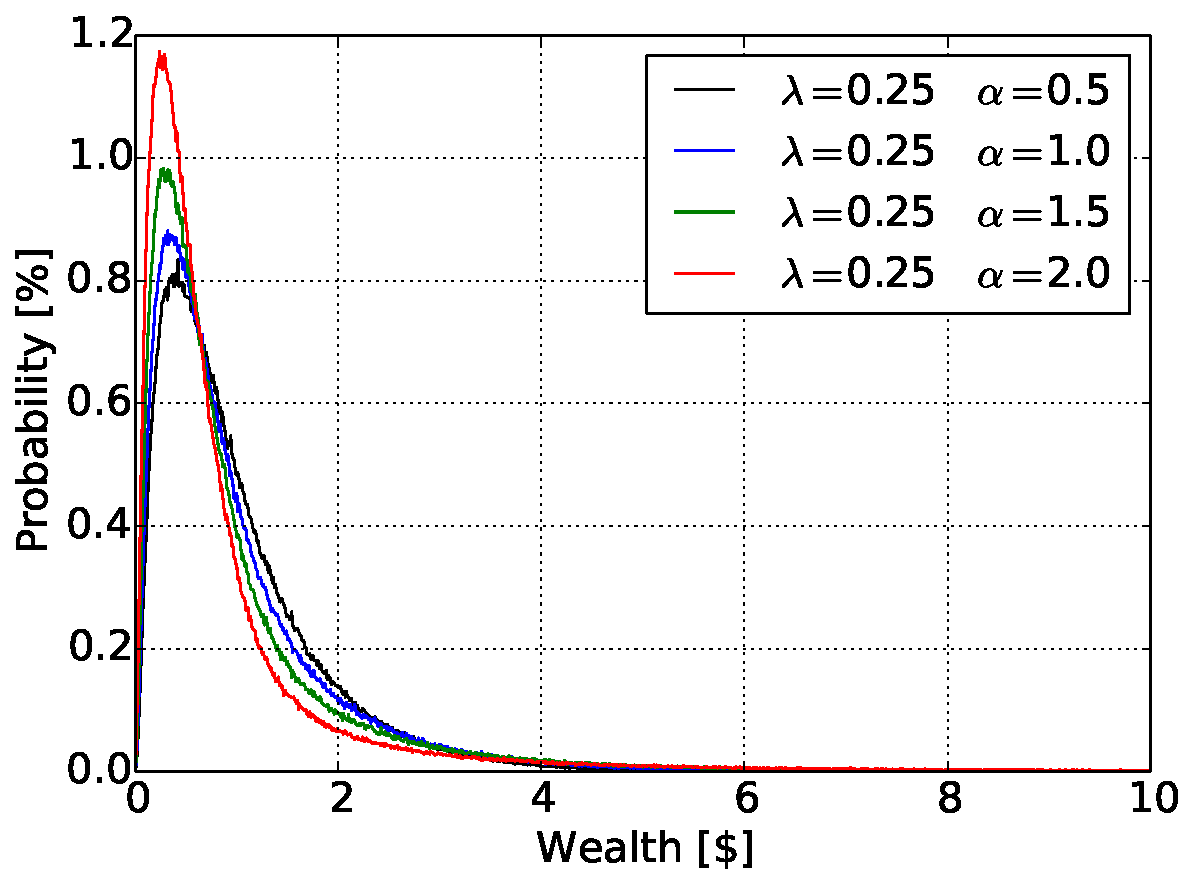
\includegraphics[width=\linewidth]{result/bilder/5d-25}
        \caption{}
    \end{subfigure}%
    ~ 
    \begin{subfigure}{0.5\textwidth}
        \centering
        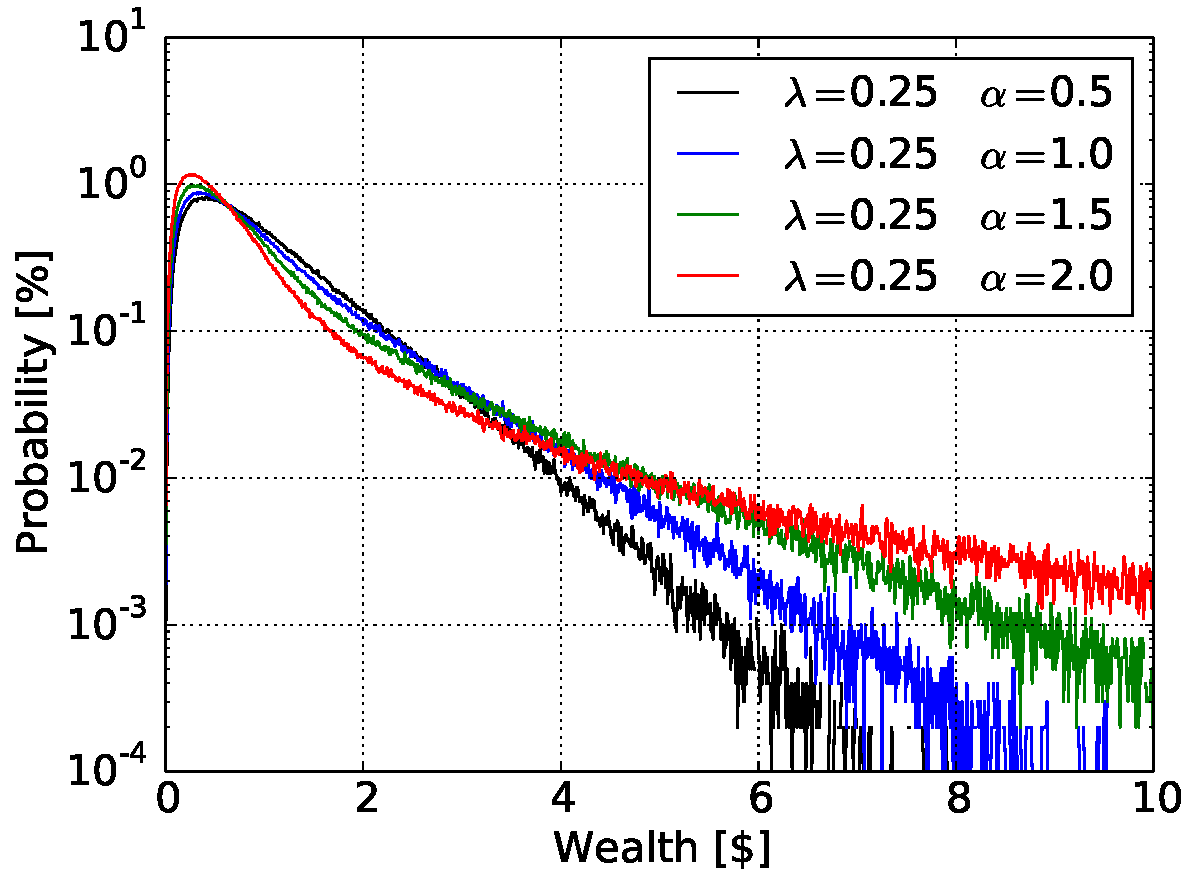
\includegraphics[width=\linewidth]{result/bilder/5d-25-log}
        \caption{}
    \end{subfigure}
    \caption{a) Shows how E behaves around $T_C$ b) Shows how |M| develops near $T_C$.}
    \label{fig:5d-25}
\end{figure}




\begin{figure}[H]
    \centering
    \begin{subfigure}{0.5\textwidth}
        \centering
        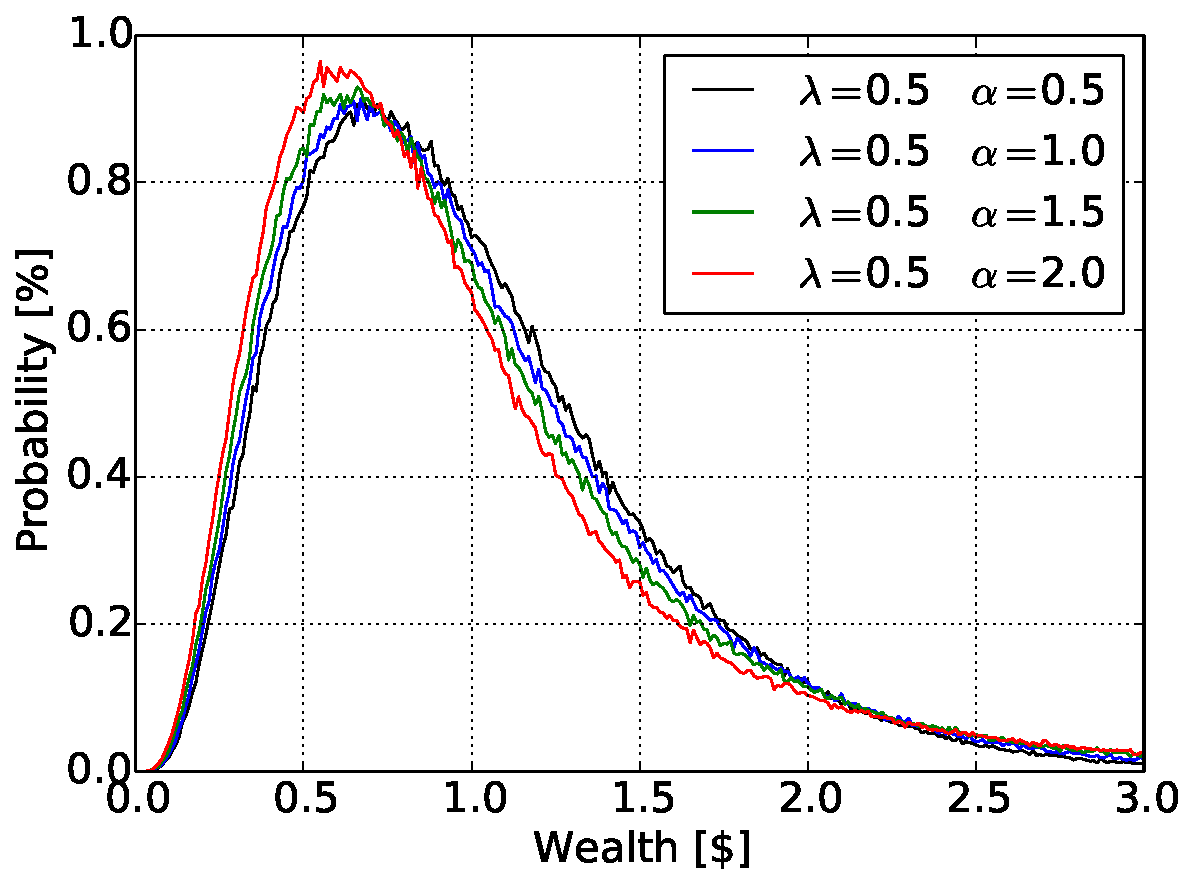
\includegraphics[width=\linewidth]{result/bilder/5d-50}
        \caption{}
    \end{subfigure}%
    ~ 
    \begin{subfigure}{0.5\textwidth}
        \centering
        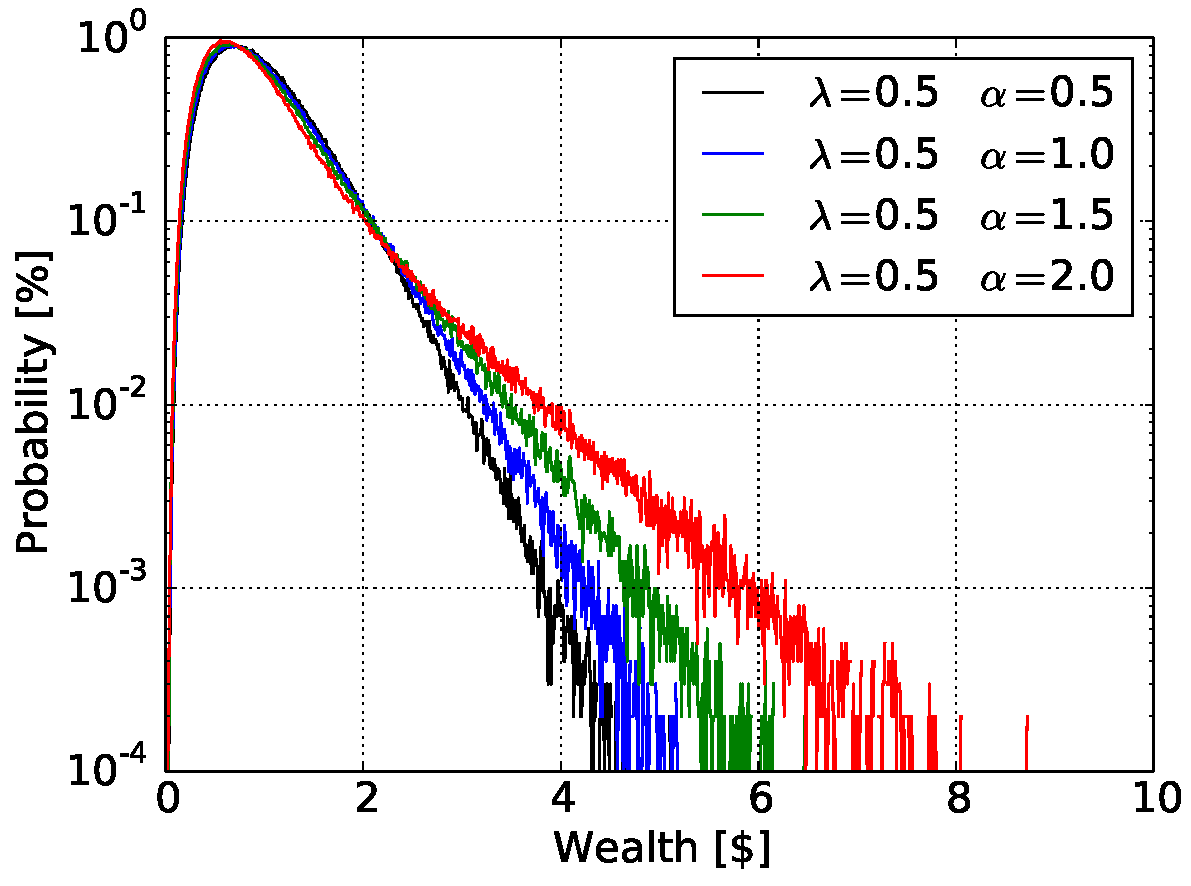
\includegraphics[width=\linewidth]{result/bilder/5d-50-log}
        \caption{}
    \end{subfigure}
    \caption{a) Shows how E behaves around $T_C$ b) Shows how |M| develops near $T_C$.}
    \label{fig:5d-50}
\end{figure}



\begin{figure}[H]
    \centering
    \begin{subfigure}{0.5\textwidth}
        \centering
        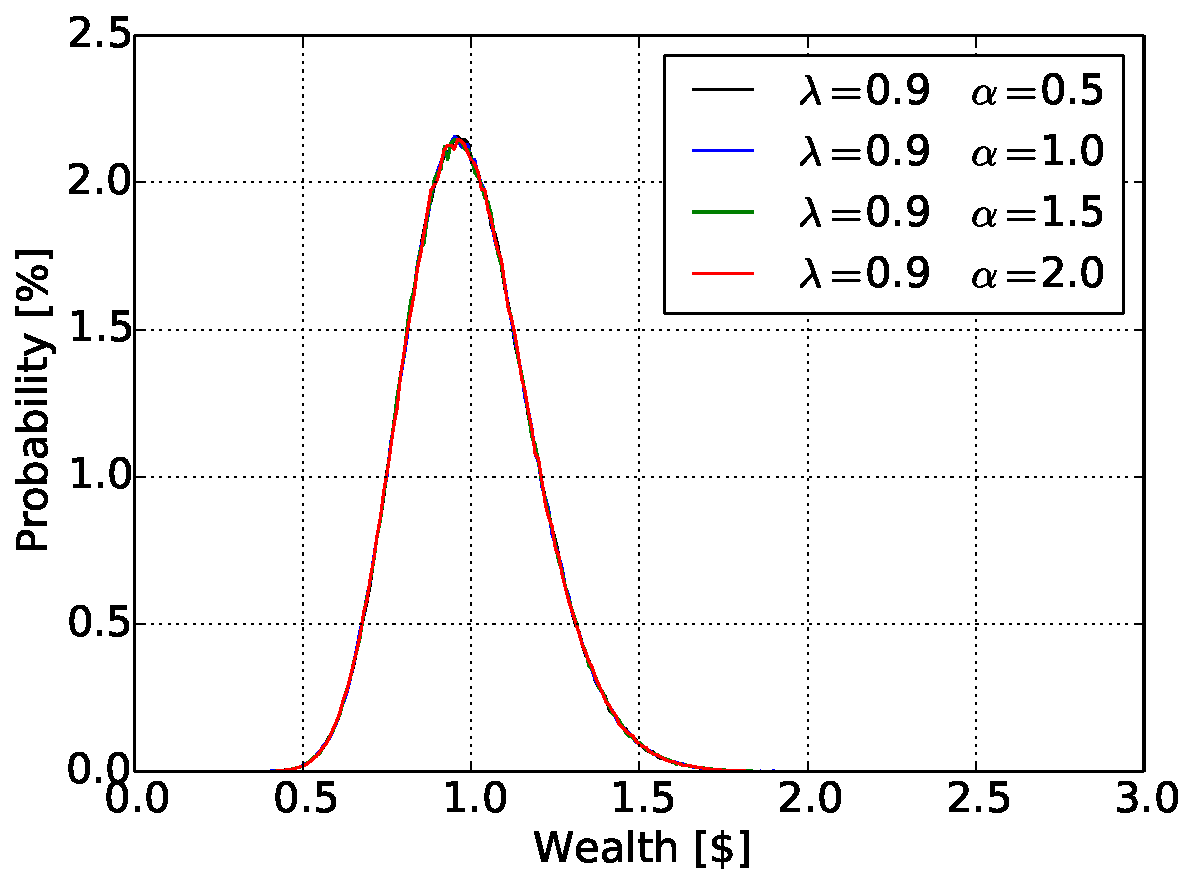
\includegraphics[width=\linewidth]{result/bilder/5d-90}
        \caption{}
    \end{subfigure}%
    ~ 
    \begin{subfigure}{0.5\textwidth}
        \centering
        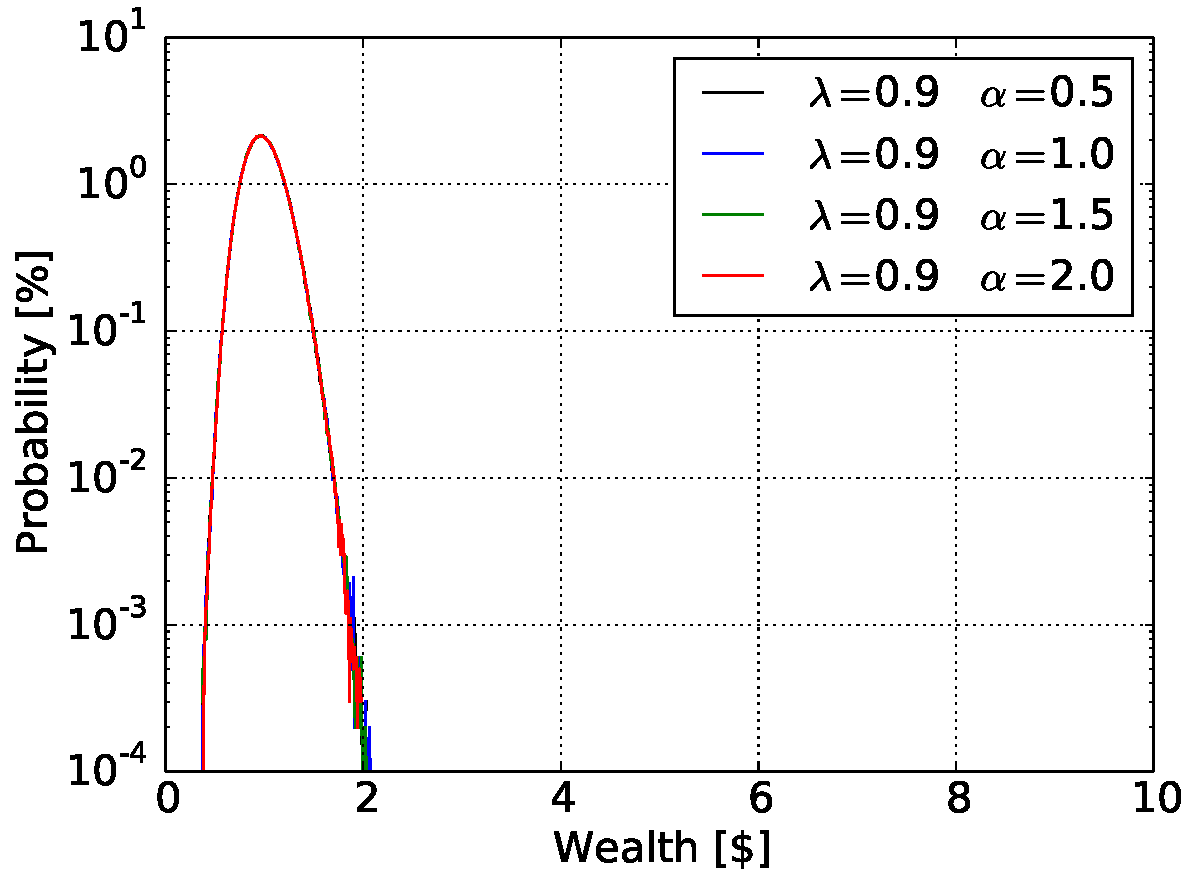
\includegraphics[width=\linewidth]{result/bilder/5d-90-log}
        \caption{}
    \end{subfigure}
    \caption{a) Shows how E behaves around $T_C$ b) Shows how |M| develops near $T_C$.}
    \label{fig:5d-90}
\end{figure}
























\pagebreak
\subsection{5e}
\begin{figure}[H]
    \centering
    \begin{subfigure}{0.5\textwidth}
        \centering
        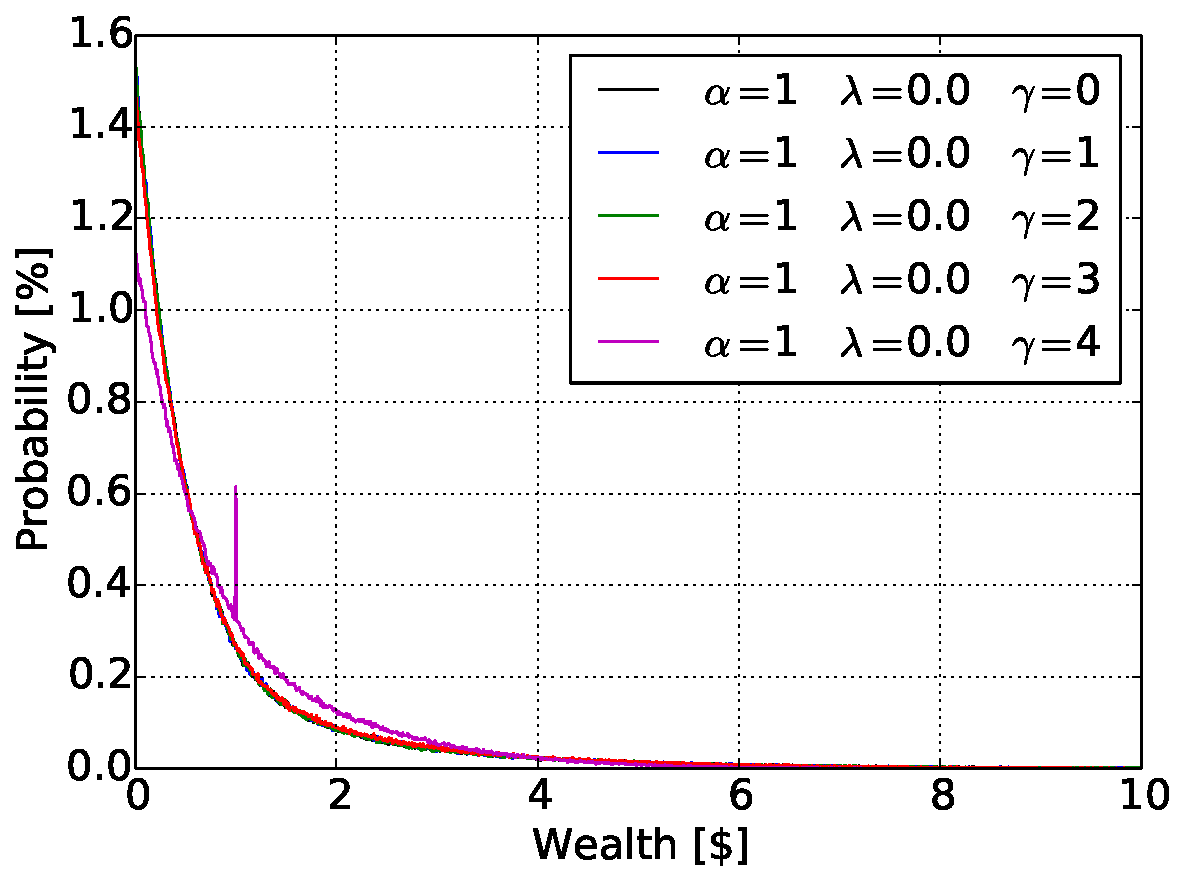
\includegraphics[width=\linewidth]{result/bilder/5e-1-00}
        \caption{}
    \end{subfigure}%
    ~ 
    \begin{subfigure}{0.5\textwidth}
        \centering
        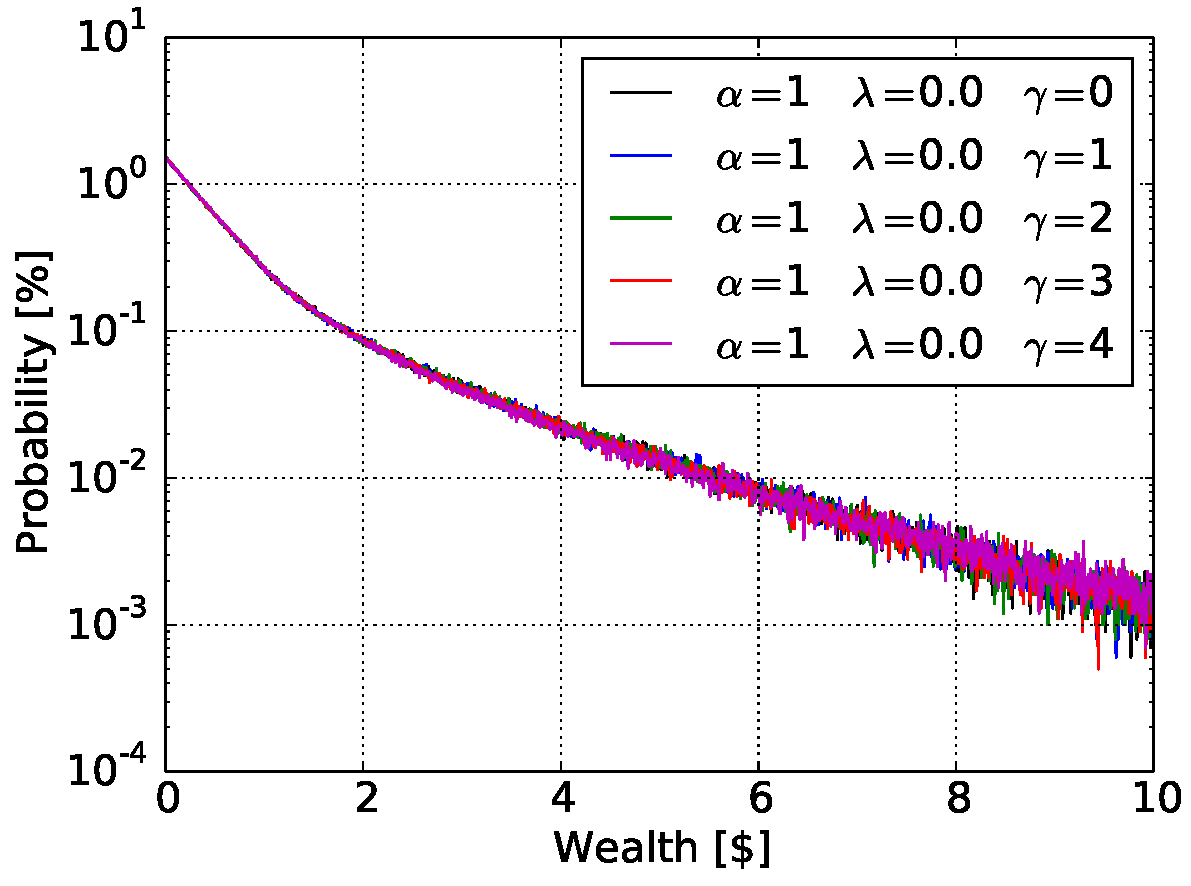
\includegraphics[width=\linewidth]{result/bilder/5e-1-00-log}
        \caption{}
    \end{subfigure}
    \caption{a) Shows how E behaves around $T_C$ b) Shows how |M| develops near $T_C$.}
    \label{fig:5e-1-00}
\end{figure}



\begin{figure}[H]
    \centering
    \begin{subfigure}{0.5\textwidth}
        \centering
        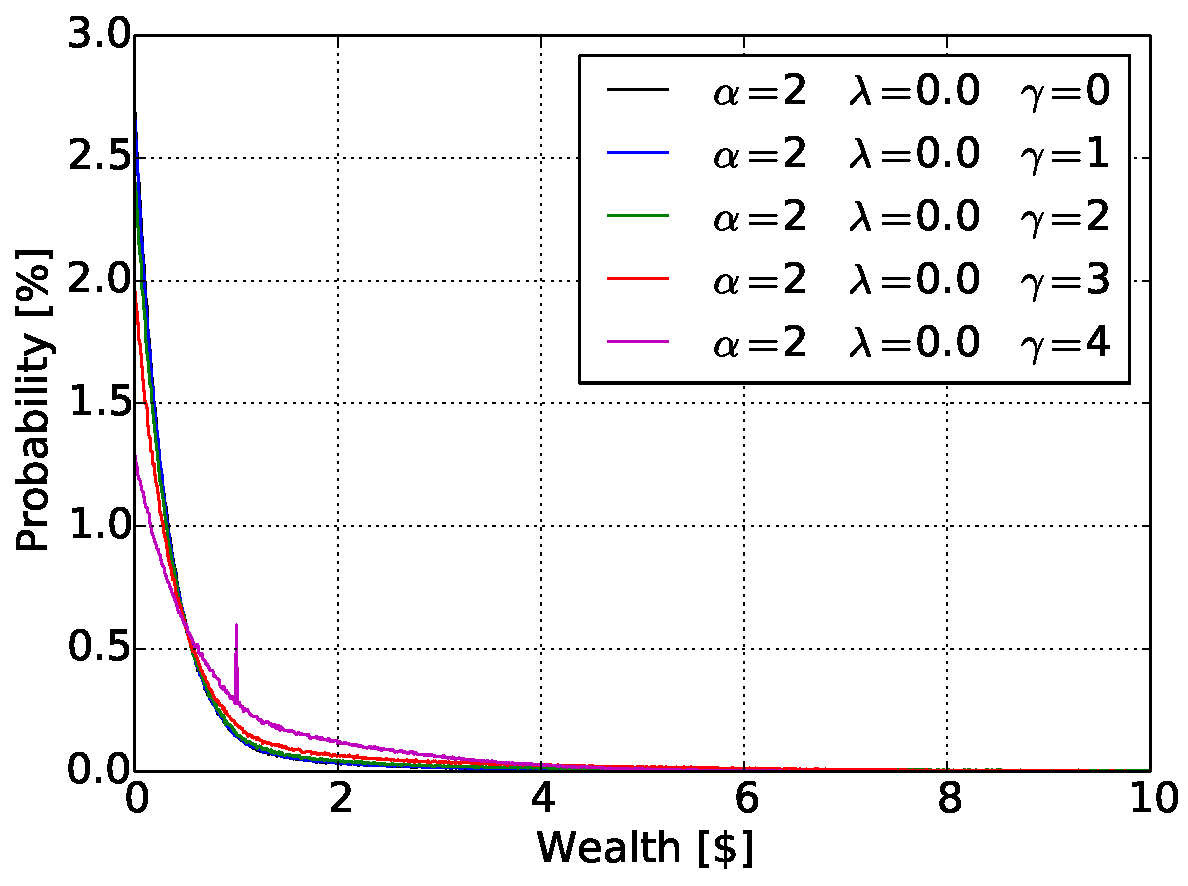
\includegraphics[width=\linewidth]{result/bilder/5e-2-00}
        \caption{}
    \end{subfigure}%
    ~ 
    \begin{subfigure}{0.5\textwidth}
        \centering
        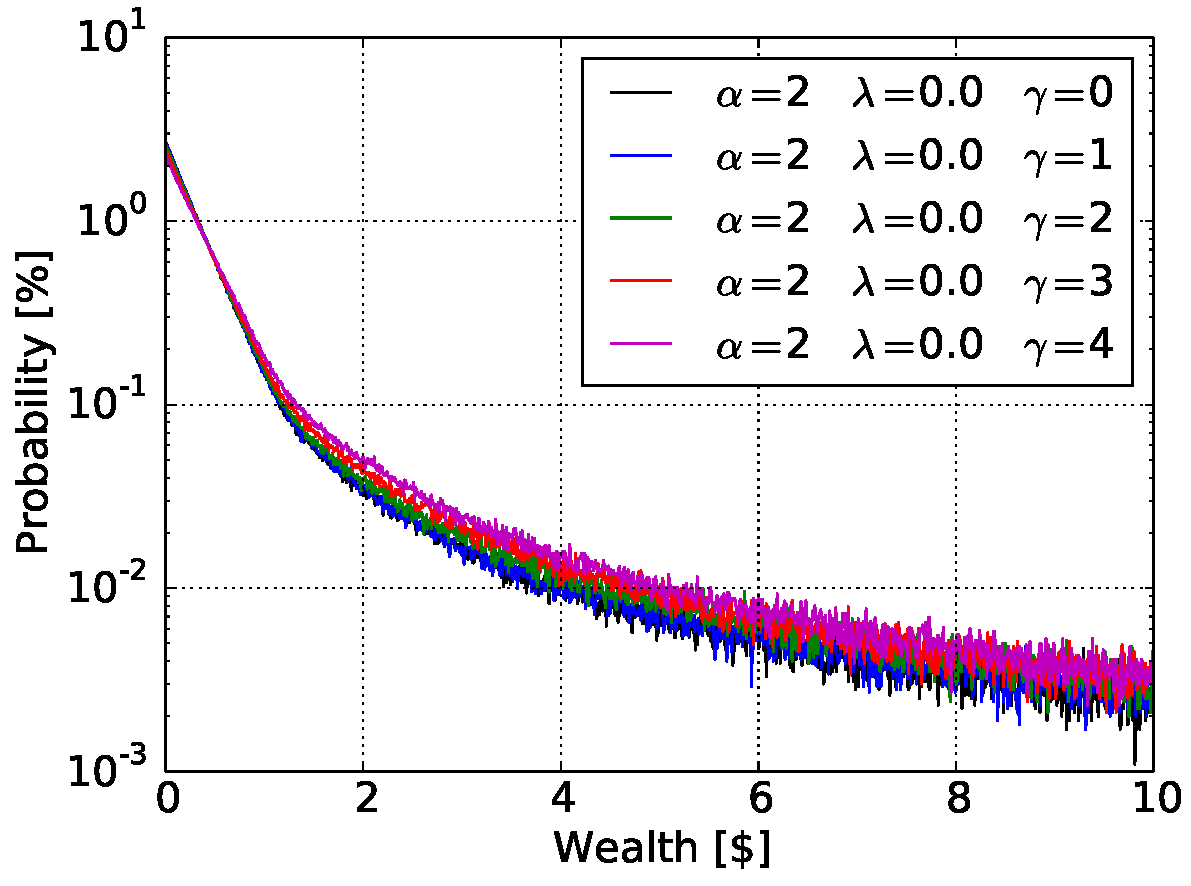
\includegraphics[width=\linewidth]{result/bilder/5e-2-00-log}
        \caption{}
    \end{subfigure}
    \caption{a) Shows how E behaves around $T_C$ b) Shows how |M| develops near $T_C$.}
    \label{fig:5e-2-00}
\end{figure}














\begin{figure}[H]
    \centering
    \begin{subfigure}{0.5\textwidth}
        \centering
        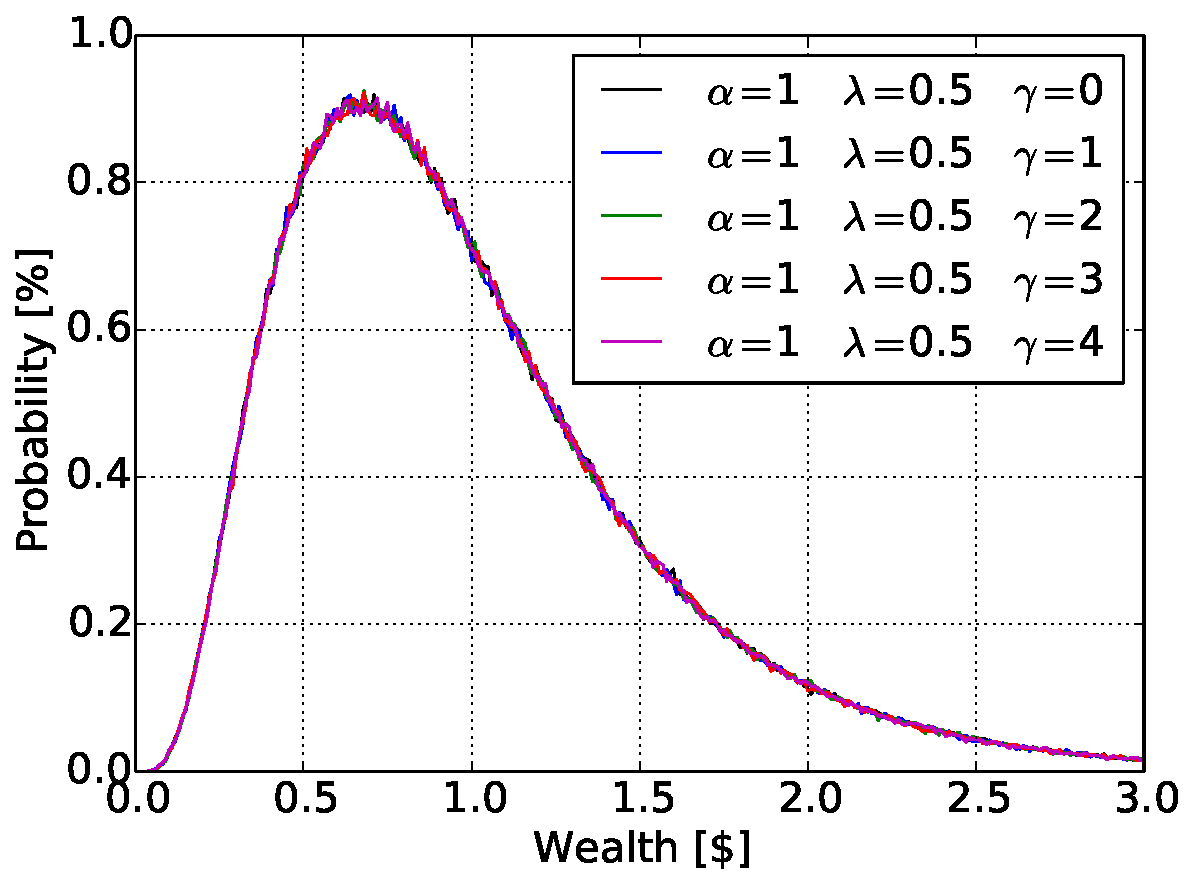
\includegraphics[width=\linewidth]{result/bilder/5e-1-50}
        \caption{}
    \end{subfigure}%
    ~ 
    \begin{subfigure}{0.5\textwidth}
        \centering
        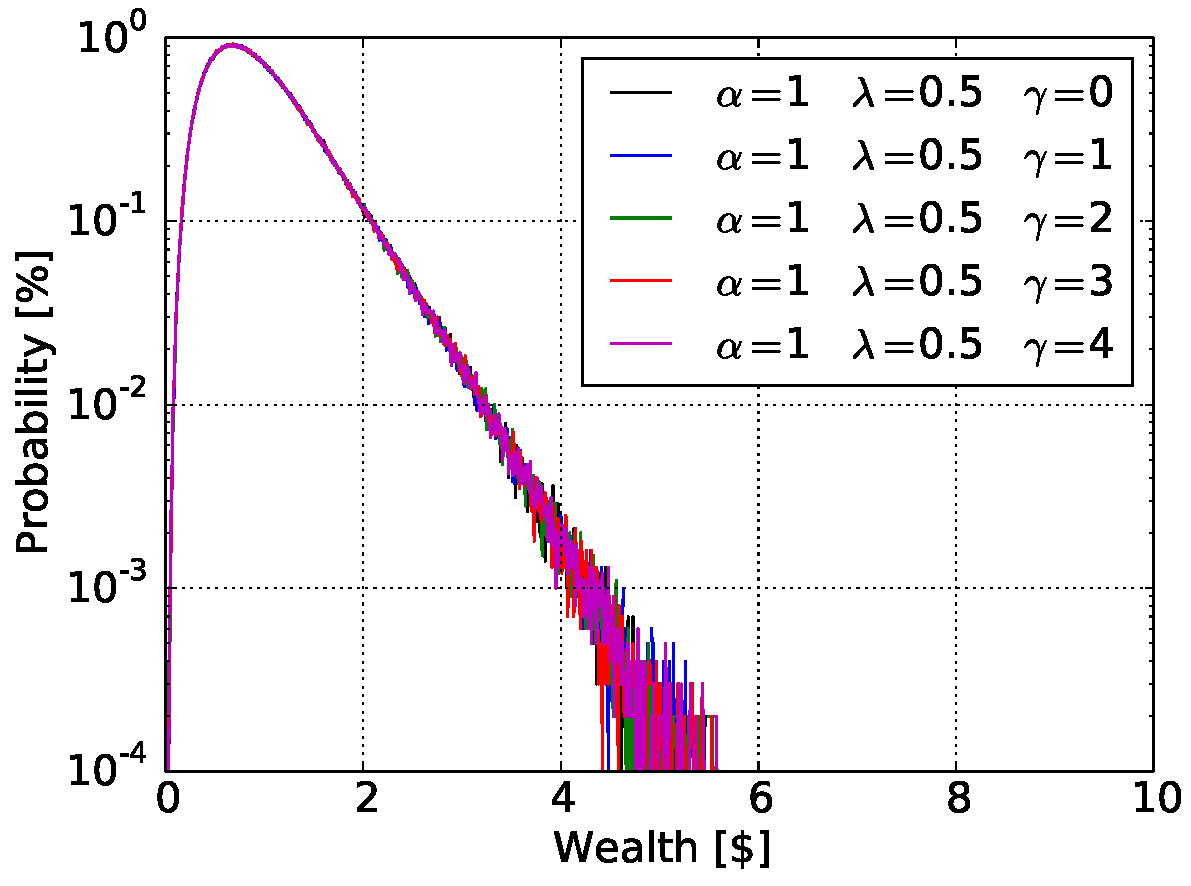
\includegraphics[width=\linewidth]{result/bilder/5e-1-50-log}
        \caption{}
    \end{subfigure}
    \caption{a) Shows how E behaves around $T_C$ b) Shows how |M| develops near $T_C$.}
    \label{fig:5e-1-50}
\end{figure}



\begin{figure}[H]
    \centering
    \begin{subfigure}{0.5\textwidth}
        \centering
        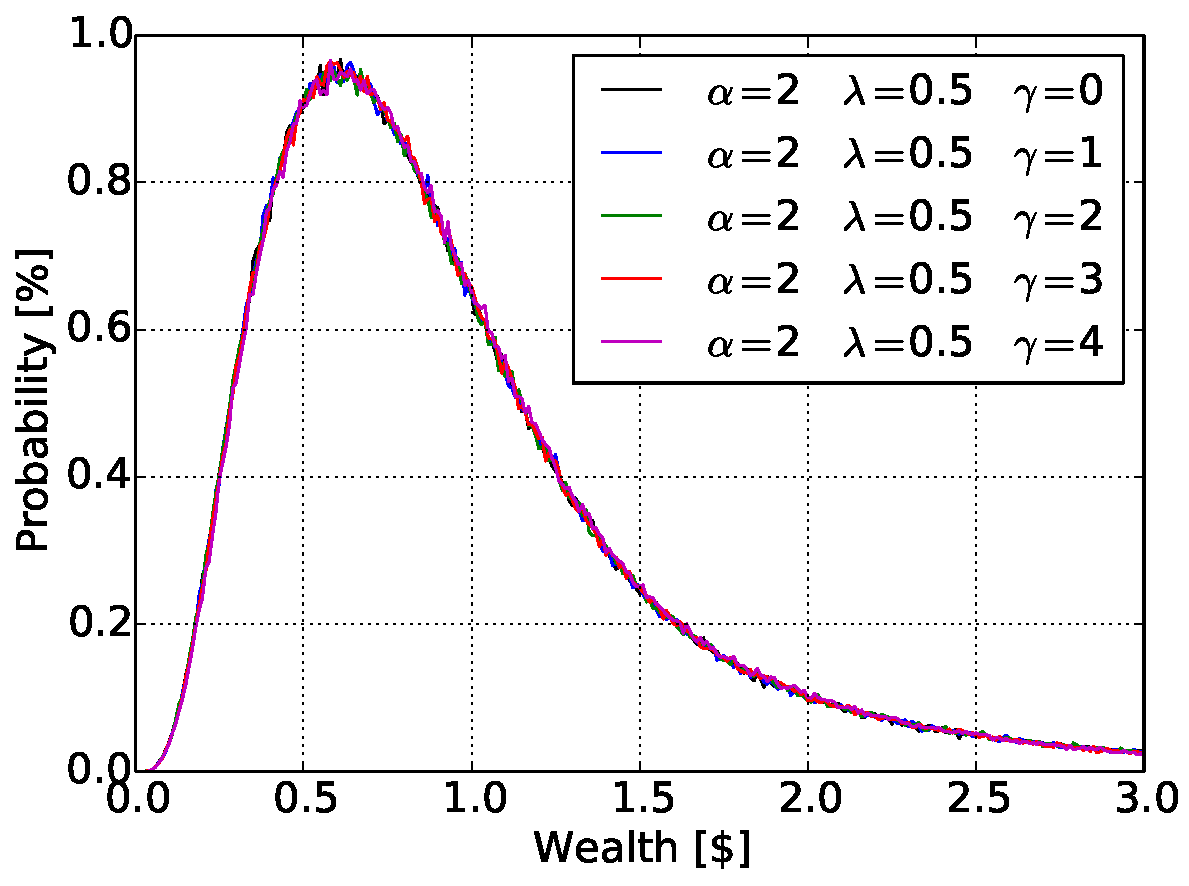
\includegraphics[width=\linewidth]{result/bilder/5e-2-50}
        \caption{}
    \end{subfigure}%
    ~ 
    \begin{subfigure}{0.5\textwidth}
        \centering
        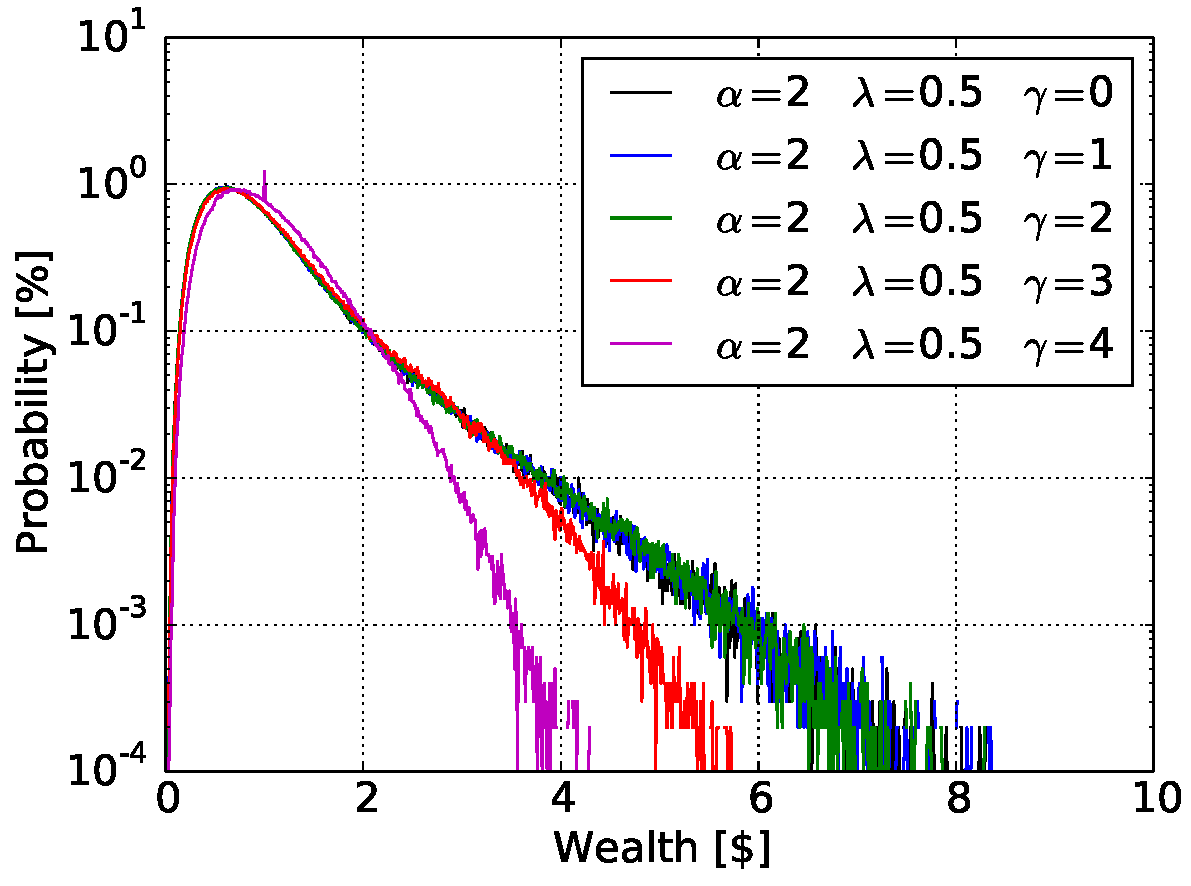
\includegraphics[width=\linewidth]{result/bilder/5e-2-50-log}
        \caption{}
    \end{subfigure}
    \caption{a) Shows how E behaves around $T_C$ b) Shows how |M| develops near $T_C$.}
    \label{fig:5e-2-50}
\end{figure}















\begin{figure}[H]
    \centering
    \begin{subfigure}{0.5\textwidth}
        \centering
        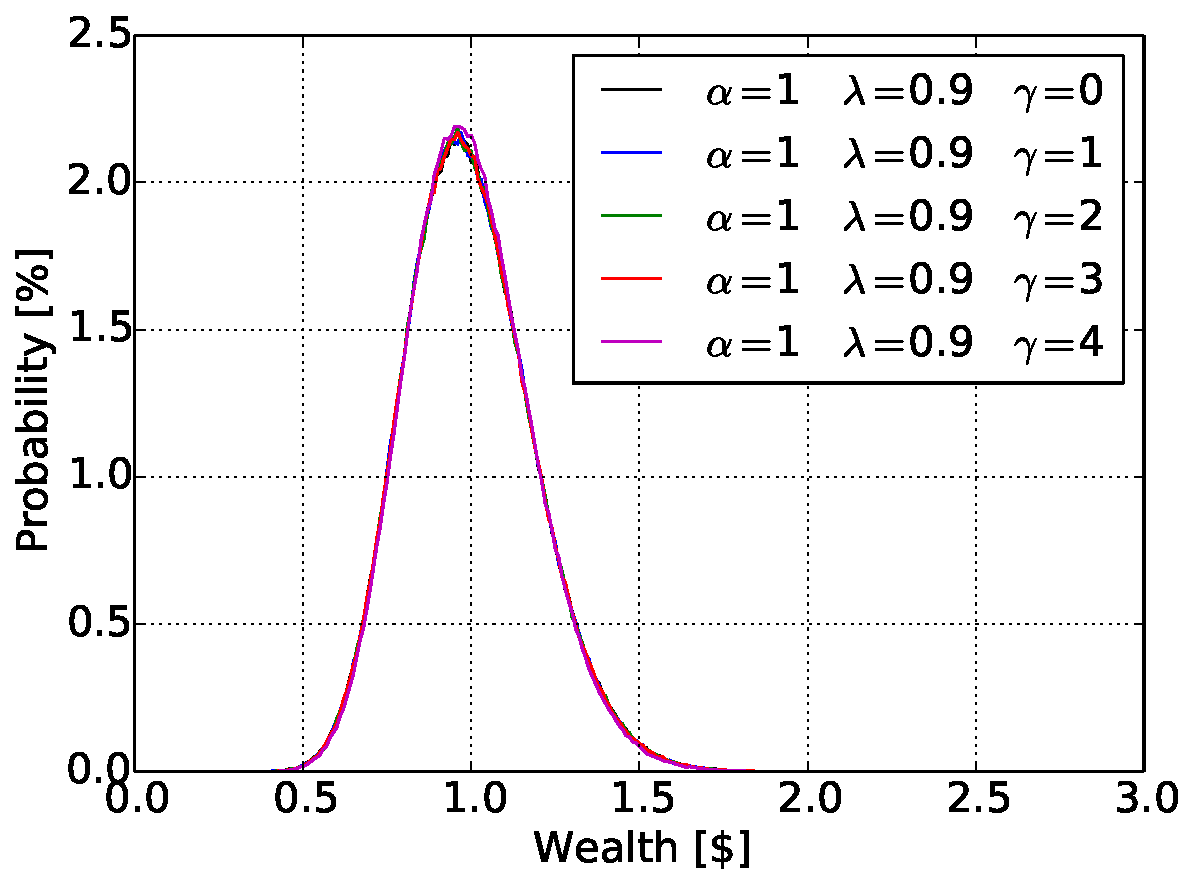
\includegraphics[width=\linewidth]{result/bilder/5e-1-90}
        \caption{}
    \end{subfigure}%
    ~ 
    \begin{subfigure}{0.5\textwidth}
        \centering
        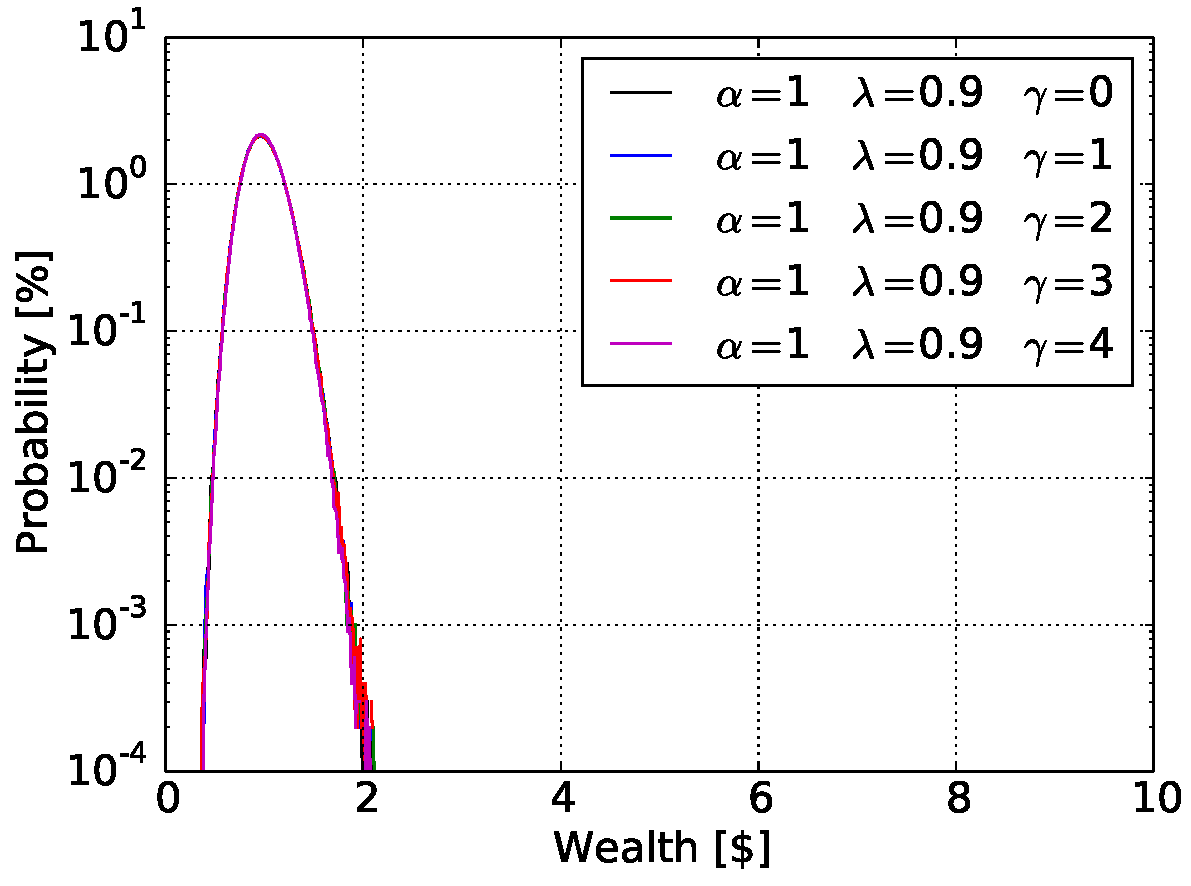
\includegraphics[width=\linewidth]{result/bilder/5e-1-90-log}
        \caption{}
    \end{subfigure}
    \caption{a) Shows how E behaves around $T_C$ b) Shows how |M| develops near $T_C$.}
    \label{fig:5e-1-90}
\end{figure}



\begin{figure}[H]
    \centering
    \begin{subfigure}{0.5\textwidth}
        \centering
        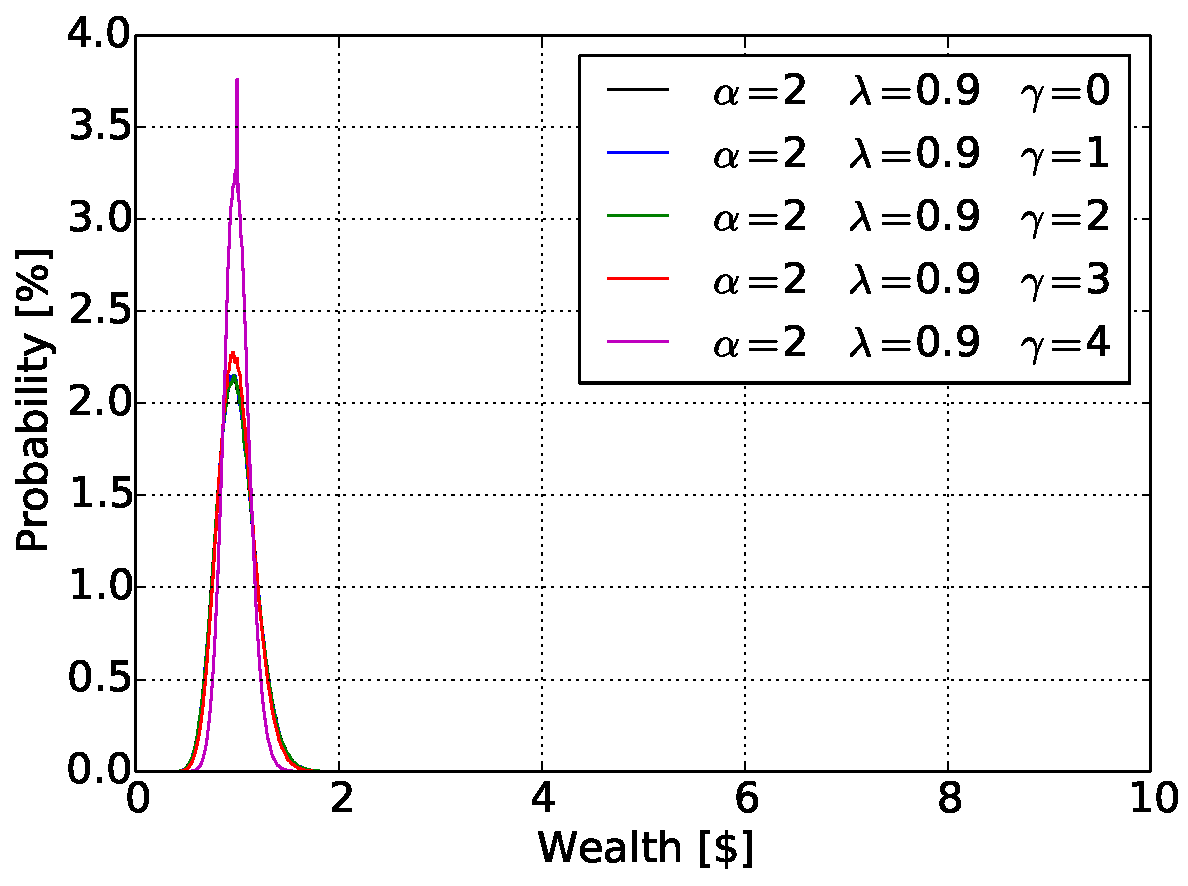
\includegraphics[width=\linewidth]{result/bilder/5e-2-90}
        \caption{}
    \end{subfigure}%
    ~ 
    \begin{subfigure}{0.5\textwidth}
        \centering
        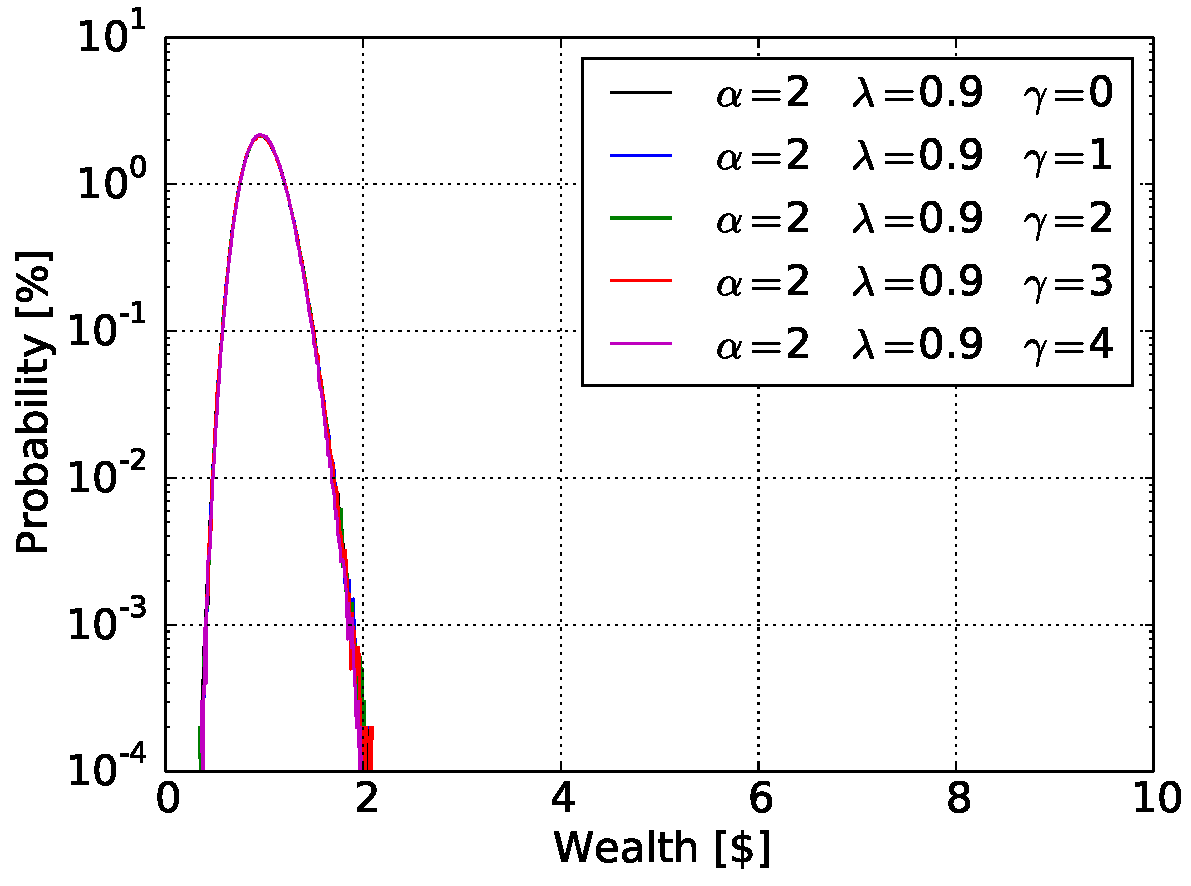
\includegraphics[width=\linewidth]{result/bilder/5e-2-90-log}
        \caption{}
    \end{subfigure}
    \caption{a) Shows how E behaves around $T_C$ b) Shows how |M| develops near $T_C$.}
    \label{fig:5e-2-90}
\end{figure}

















%\pagebreak
%\section{Discussion}
%\input{discussion/discussion}


\section{Conclusion}
In this project a have created a generalized closed transaction model. Agents and the amount of wealth that is traded is randomly selected. A saving term was implemented which turned out to be positive for must agent. Different probability terms were introduced to the model. \todo{MIKAEL, skriv tre setninger om hoved essensen av hva du skrev i resultdelen.}
\\
\\
For future work one should try to make the trade ratio time dependent. The denominator in the trade ratio becomes larger over time, but a more realistic model would make the agents only care about the last part of the transaction they did. The effect of taxing or universal basic income would also be interesting to see, but this was to much work for this project. 


\section{References}
\printbibliography

\section{Appendix}\label{sec:appendix}
\input{appendix/appendix}



%\begin{align*}
%&n \qquad &2^n - (-1)^n\\
%&n+1 \qquad &2^{n+1} - (-1)^{n+1} \\
%& &= 2(2^{n}) - (-1)^{n+1}\\
%& &= 2(2^{n} + (-1)^n  + (-1)^{n+1}) - (-1)^{n+1}\\
%& &= 2(2^{n} + (-1)^n  - (-1)^{n}) - (-1)^{n+1}\\
%& &= 2(2^{n}- (-1)^{n}) + 2(-1)^n  + (-1)^{n}\\
%& &= 2(2^{n}- (-1)^{n}) + 3(-1)^n \\
%\end{align*}



%\begin{tabular}{|c|c|c|c|c|c|c|}
%	\hline 
%	n & General & Specific & LU & fastest & slowest & $\frac{slowest}{fastest}$\\ 
%	\hline
%	10 & 6.5e-05 & 5e-06 & 4e-05 & Specific & General & 13.0\\ 
%	\hline 
%	100 & 7.5e-05 & 8e-06 & 0.0023 & Specific & LU & 287.5\\ 
%	\hline 
%	1000 & 0.00014 & 4e-05 & 0.26 & Specific & LU & 6500\\ 
%	\hline
%	10000 & 0.0007 & 0.0005 & 142.5 & Specific & LU & 285000 \\ 
%	\hline
%\end{tabular}

%\begin{figure}[H]
%		\centering
%		\includegraphics[width=0.7\linewidth]{ab.png}
%		\caption{Atomene er gule kuler, de elementære vektorene er blå og a vektorene er grønne.}
%		\label{fig:ab}
%\end{figure}



\end{document}
